\documentclass[twoside,a4paper,11pt]{book}
\usepackage[english]{babel}

\usepackage[utf8]{inputenc}
\usepackage[T1]{fontenc}
\usepackage{url}
\usepackage[pdftex]{graphicx}
\usepackage{a4wide}
\usepackage{geometry}
\usepackage[backend=bibtex]{biblatex}
\usepackage{hyperref}
\usepackage{subfiles}
\usepackage[normalsize]{subfigure}
\usepackage{color}
\usepackage{amsmath}
\usepackage{amsfonts}
\usepackage[normalem]{ulem}
\usepackage{float}
\usepackage{enumitem}
\usepackage{mathtools}
\usepackage{listings}
\usepackage{textcomp}
\usepackage{tikz}
\usepackage{verbatim}
\usepackage{forest}
\usepackage{fontawesome}

% For notes, corrections and suggestions
\definecolor{GRCOLOR}{rgb}{1,0.2,0.5}
\definecolor{ODRCOLOR}{rgb}{0.2,0.75,0.25}
\definecolor{LRCOLOR}{rgb}{0.2,0.3,1}
\definecolor{MyDarkRed}{rgb}{0.6,0,0.0}

\newcommand{\GR}[1] { \mycomment[PT]{#1}{GRCOLOR}}
\newcommand{\ODR}[1]{ \mycomment[ODR]{#1}{ODRCOLOR}}
\newcommand{\LR}[1]{ \mycomment[SM]{#1}{LRCOLOR}}

\newcommand{\newGR}[1]{\textcolor{PTCOLOR}{\uline{#1}}} %\sout}
\newcommand{\delGR}[1]{\textcolor{PTCOLOR}{\sout{#1}}} %\sout}
\newcommand{\newODR}[1]{\textcolor{ODRCOLOR}{\uline{#1}}} %\sout}
\newcommand{\delODR}[1]{\textcolor{ODRCOLOR}{\sout{#1}}} %\sout}
\newcommand{\newLR}[1]{\textcolor{SMCOLOR}{\uline{#1}}} %\sout}
\newcommand{\delLR}[1]{\textcolor{SMCOLOR}{\sout{#1}}} %\sout}
\newcommand{\note}[1]{\textcolor{MyDarkRed}{#1}} %\sout}
\newcommand{\deletenote}[1]{\textcolor{MyDarkRed}{\sout{#1}}} %\sout}



\setcounter{tocdepth}{4}
\setcounter{secnumdepth}{4}

% For using margin notes instead of marginpar
\usepackage{marginnote}
% Margin notes smaller that default
\renewcommand*{\marginfont}{\footnotesize}
\newcommand{\myparagraph}[1]{\paragraph{#1}\mbox{}\\}

\addto\captionsenglish{\renewcommand{\chaptername}{Capítulo}}
\addto\captionsenglish{\renewcommand{\contentsname}{Índice}}
\addto\captionsenglish{\renewcommand{\listfigurename}{Lista de figuras}}

\lstset{
    backgroundcolor=\color[rgb]{0.95, 0.95, 0.95},
    tabsize=2,
    rulecolor=,
    basicstyle=\scriptsize,
    upquote=true,
    aboveskip={1.5\baselineskip},
    columns=fixed,
    showstringspaces=false,
    extendedchars=true,
    breaklines=true,
    prebreak = \raisebox{0ex}[0ex][0ex]{\ensuremath{\hookleftarrow}},
    frame=single,
    showtabs=false,
    showspaces=false,
    showstringspaces=false,
    identifierstyle=\ttfamily,
    keywordstyle=\color[rgb]{1.0,0,0},
    keywordstyle=[1]\color[rgb]{0,0,0.75},
    keywordstyle=[2]\color[rgb]{0.5,0.0,0.0},
    keywordstyle=[3]\color[rgb]{0.127,0.427,0.514},
    keywordstyle=[4]\color[rgb]{0.4,0.4,0.4},
    commentstyle=\color[rgb]{0.133,0.545,0.133},
    stringstyle=\color[rgb]{0.639,0.082,0.082},
}

\lstdefinestyle{java} {
    language=Java,
    morekeywords={record, var}
}

\newcommand{\basictree}[1]{\begin{forest}
    for tree={
        font=\ttfamily,
        grow'=0,
        child anchor=west,
        parent anchor=south,
        anchor=west,
        calign=first,
        edge path={
            \noexpand\path [draw, \forestoption{edge}]
            (!u.south west) +(7.5pt,0) |- node[fill,inner sep=1.25pt] {} (.child anchor)\forestoption{edge label};
        },
        before typesetting nodes={
            if n=1
                {insert before={[,phantom]}}
                {}
        },
        fit=band,
        before computing xy={l=15pt},
    }
    #1
\end{forest}}

\DeclareGraphicsExtensions{.png, .jpg, .pdf, .eps, .tiff}
\DeclareGraphicsRule{.eps}{pdf}{.pdf}{pdf}
\pdfcompresslevel=9
\geometry{a4paper, left=2.6cm, right=2.2cm, top=3.0cm, bottom=3.0cm}
\linespread{1.2}
\setlength{\parskip}{1ex plus 0.5ex minus 0.2ex}

\bibliography{main}

\begin{document}
    \thispagestyle{empty}


\includegraphics{images/URJC_logo}
\vspace{2cm}

\begin{center}
	\large{\textbf{ESCUELA TÉCNICA SUPERIOR DE INGENIERÍA INFORMÁTICA}}
	\vspace{5mm}

 	{\Large {Grado en Ingeniería de Computadores}}
    \\
  	\vspace{34mm}
	{\large {\bf TRABAJO FIN DE GRADO}}
  	\vspace{10mm}
    \\
  	{\Large {{\Huge {
  		JAMS: entorno moderno de desarrollo para MIPS32 con un enfoque educativo
	}} \\[1cm] }}
  	\vspace{2cm}
	{\large {
        \textbf{Autor}: Gael Rial Costas\\
        \textbf{Tutores}:\\
        Luis Rincón Córcoles\\
        Óscar David Robles Sánchez\\
  	}}
	\vspace{10mm}
  	{\large {Curso académico 2021/2022}}
  	\vspace{1cm}
\end{center}

    \clearpage
    \thispagestyle{empty}
    \vspace{5cm}
    \frontmatter
    \chapter{Resumen} \label{ch:resumen}

Este Trabajo \delODR{de} Fin de Grado contempla el diseño y desarrollo de \textit{JAMS},
un entorno de desarrollo integrado moderno, ligero y altamente modificable
para proyectos en lenguaje ensamblador.
El entorno de desarrollo incorpora por defecto un editor, ensamblador y simulador
para la arquitectura \textit{MIPS32}, con un enfoque educativo.
Para ello, la aplicación presenta varias herramientas que permiten
visualizar el estado del proyecto desde diferentes puntos de vista.\\
Con esto, se pretende contribuir \delODR{en}\newODR{a} una enseñanza de mejor calidad para
los alumnos que cursan alguna asignatura relacionada con arquitectura\delODR{s}\newODR{ de computadores},
procesadores o lenguajes de programación de bajo nivel.

    \chapter{Abstract} \label{ch:abstract}

This Bachelor's Thesis to obtain the Degree of Coputing Engineering contemplates the design and development of \textit{JAMS},
a modern, lightweight and highly modifiable integrated
development environment for assembly language projects.
The development environment incorporates by default an editor,
assembler and simulator for the MIPS32 architecture, with an educational approach.
For this purpose, the application presents several tools that allow visualizing
the project status from different points of view.
With this, it is intended to contribute to a better quality
teaching for students taking a subject related to computer architecture,
processors or low-level programming languages.

    \tableofcontents
    \listoffigures
    \mainmatter
    \chapter{Descripción del problema} \label{ch:descripcion-del-problema}


\section{Definición de conceptos}\label{sec:definicion-de-conceptos}

\subsection{La arquitectura \textit{MIPS}}\label{subsec:la-arquitectura-mips}

Se conoce con el nombre de \textbf{procesadores \textit{MIPS}}
\footnote{Creado por \emph{MIPS Computer Systems}, en la actualidad \emph{MIPS Technologies}}
a una familia de microprocesadores que implementan
la arquitectura \textit{RISC} del mismo nombre.
Aunque esta arquitectura no ha tenido un gran éxito en los computadores personales, sí ha gozado de fama en
sistemas empotrados, enrutadores, videoconsolas como la \textit{Nintendo 64} o la \textit{PlayStation 2},
y en máquinas utilizadas en diferentes aplicaciones, como las estaciones \textit{SGI IRIS 4D}
creadas por \textit{Silicon Graphics, Inc.} y empleadas en la industria cinematográfica para
la creación de animaciones y la generación de efectos especiales.

Su simple diseño y baja curva de aprendizaje hace a esta arquitectura ideal para introducir a los alumnos
a los lenguajes ensambladores.

\subsection{\textit{IDEs}: entornos de desarrollo integrados}\label{subsec:ides-entornos-de-desarrollo-integrados}

Un \textbf{entorno de desarrollo integrado} (\textit{IDE, Integrated Development Environment}) es una aplicación
informática con diversas herramientas empleadas en el desarrollo, construcción y depuración de \textit{software}.
Un \textit{IDE} suele estar desarrollado con dos objetivos clave en mente: maximizar la productividad del
desarrollador y evitar que este tenga que utilizar herramientas externas en su trabajo.

Existe una gran variedad de entornos de desarrollo en el mercado.
Estos se pueden clasificar de diferentes maneras.

\textbf{Según su propósito:}
\begin{itemize}
    \item \textbf{Entornos de desarrollo específicos:} son entornos pensados para el desarrollo en una
    tecnología concreta.
    Algunos ejemplos son \textit{NetBeans}, \textit{CLion} o \textit{Android Studio}.
    \item \textbf{Entornos de desarrollo generales:} son entornos que no se centran en una tecnología en concreto.
    Algunos ejemplos son \textit{IntelliJ IDEA}\cite{INTELLIJIDEA},
    \textit{Eclipse}\cite{ECLIPSE} o \textit{Microsoft Visual Studio}\cite{VISUALSTUDIO}
\end{itemize}

\textbf{Según su complejidad:}
\begin{itemize}
    \item \textbf{Entornos de desarrollo complejos:} son aplicaciones pesadas con una gran cantidad de
    características y funcionalidades.
    Algunos ejemplos son \textit{IntelliJ IDEA},
    \textit{Microsoft Visual Studio} o \textit{Eclipse}.
    \item \textbf{Entornos de desarrollo ligeros:} son aplicaciones que ocupan muy poco espacio, donde
    las características más avanzadas suelen ser componentes descargables.
    Algunos ejemplos son \textit{Visual Studio Code}\cite{VISUALSTUDIOCODE},
    \textit{Atom}\cite{ATOM} o \textit{Notepad++}\cite{NOTEPADPP}.
\end{itemize}

\subsection{Simuladores y emuladores}
\label{subsec:simuladores-y-emuladores}

Tanto un simulador como un emulador puede definirse como un
programa de computador que imita el funcionamiento de uno o varios
componentes \textit{hardware}.
Un emulador o simulador imita a una arquitectura, permitiendo
ejecutar aplicaciones ajenas a la arquitectura del computador anfitrión.

Es importante diferenciar los conceptos de \textbf{simulación}
y \textbf{emulación} a la hora de crear un programa que ejecute
código de arquitecturas externas.
La diferencia entre los simuladores y emuladores se manifiesta
en la manera en la que se implementan.

Un emulador tiene como objetivo \textbf{imitar el resultado}
que la arquitectura imitada produce al ejecutar un programa, sin tener
en cuenta el proceso interno que produce dicho resultado.
Los emuladores tienden a ser rápidos, intentando producir el resultado
de la manera más rápida y fiel posible.

Los simuladores tienen como objetivo \textbf{imitar el proceso}
que produce el resultado, simulando todos los componentes de la arquitectura.
Los simuladores tienden a ser más lentos que los emuladores, pero son más
adecuados para desarrollar y depurar aplicaciones para la arquitectura
imitada aunque no se disponga físicamente del \textit{hardware}.


\section{Descripción del problema}\label{sec:descripcion-del-problema}

Como se verá más adelante, los simuladores de la arquitectura \textit{MIPS} tuvieron
un auge importante a principios del milenio, con herramientas como \textit{MARS}\cite{MARS}
o \textit{EduMIPS64}\cite{EDUMIPS64}.
Estas herramientas estaban centradas principalmente en el \textbf{ámbito educativo}, proporcionando
interfaces sencillas y pocas herramientas.
Con el paso de los años, estas herramientas han quedado obsoletas, impidiendo desarrollar aplicaciones
en ensamblador \textit{MIPS32} de una manera cómoda.

Los principales problemas que presentan estas aplicaciones son los siguientes:
\begin{itemize}
    \item \textbf{Falta de herramientas}: los entornos de desarrollo \textit{MIPS} sufren de una
    carencia grave de herramientas importantes.
    Este problema afecta principalmente a programas como \textit{EduMIPS64}, donde no existe un editor de texto y
    el ensamblador es una aplicación separada que require la línea de comandos para funcionar.
    \item \textbf{Falta de estructura de proyecto}: a excepción de MARS, que lo hace de forma muy rudimentaria,
    ninguna aplicación actual presenta una estructura
    de proyecto, indispensable para el desarrollo de aplicaciones medianas y grandes.
    \item \textbf{Falta de personalización}: al ser aplicaciones muy sencillas, ninguna permite
    personalizar la apariencia de la interfaz.
    \item \textbf{Obsolescencia}: las aplicaciones están desarrolladas con tecnologías antiguas,
    con interfaces similares a las de los programas de principio de siglo.
    \item \textbf{Falta de capacidad de expansión}: el problema más grave que presentan estas aplicaciones
    es la poca capacidad de expansión de sus características, impidiendo que otros desarrolladores
    añadan nuevas funcionalidades de manera sencilla.
    \textit{MARS} es de los pocos entornos de desarrollo que permite expandir
    sus características mediante componentes,
    aunque su funcionamiento es muy rudimentario: el usuario debe modificar el archivo ejecutable
    para añadir nuevas herramientas.
\end{itemize}


\section{Objetivos}\label{sec:objetivos}

El objetivo principal de este proyecto es el desarrollo de \textbf{\textit{JAMS}
(\textit{Just Another MIPS Simulator})}, un \textbf{entorno de desarrollo integrado ligero, expandible y moderno}
centrado en los lenguajes ensambladores y, más concretamente,
en el lenguaje ensamblador de la arquitectura \textit{MIPS}.
Específicamente, en este apartado se detallarán diferentes objetivos.

\subsection{Investigar sobre las tecnologías más adecuadas para el desarrollo}
\label{subsec:investigar-sobre-las-tecnologias-mas-adecuados-para-el-desarrollo}

La tecnología usada en un proyecto tiene mucho peso en el resultado final.
Por ello, se debe buscar un conjunto de tecnologías que permitan crear una aplicación
moderna, multiplataforma y expandible.

Este objetivo puede separarse en dos pasos:
\begin{itemize}
    \item Elegir un lenguaje de programación con capacidad para crear aplicaciones modernas,
    que permita cargar código externo a voluntad y que tenga un buen rendimiento
    tanto en la ejecución como en el desarrollo.
    \item Seleccionar un \textit{framework} de desarrollo de aplicaciones de escritorio
    que permita desarrollar aplicaciones modernas y de gran
    calidad, dentro de las posibilidades del lenguaje de
    programación seleccionado.
\end{itemize}

\subsection{Crear un entorno base y un \textit{framework} que permita implementar diferentes herramientas}
\label{subsec:crear-un-entorno-base-y-un-framework-que-permita-implementar-diferentes-herramientas}

\textit{JAMS} pretende ser un entorno de desarrollo completamente modificable.
La mejor manera para conseguirlo es crear una base genérica
que se pueda ajustar posteriormente al desarrollo de una tecnología en concreto.

Esta base debe poder personalizar cualquier aspecto de la aplicación,
desde modificar simples mensajes y parámetros hasta añadir nuevas herramientas.
Estas modificaciones pueden venir de diferentes fuentes como
los paquetes de idiomas, los paquetes de temas y los complementos.

Por último, \textit{JAMS} debe permitir al usuario configurar los parámetros
de la aplicación de manera sencilla, proporcionando una interfaz de configuración
cómoda de utilizar.

Para conseguir este resultado, se proponen los siguientes subobjetivos:
\begin{itemize}
    \item Desarrollar una aplicación base en conjunto con una \textit{API} que pueda
    utilizarse por las diferentes herramientas para tecnologías concretas.
    \item Desarrollar e investigar diferentes formatos que permitan guardar
    y modificar los diferentes elementos estáticos de la aplicación, como
    los idiomas, los temas y la configuración, por ejemplo.
\end{itemize}

Este objetivo está relacionado con los
objetivos del Trabajo Fin de Grado del Grado en
Diseño y Desarrollo de Videojuegos de
la misma autoría que este Trabajo Fin de Grado:
desarrollar un \textbf{sistema de carga
dinámica de componentes} que permita al usuario activar y desactivar
componentes a voluntad sin tener que reiniciar la aplicación, así como
desarrollar tecnologías que permitan \textbf{modificar}
todos los aspectos de \textit{JAMS} mediante componentes.

\subsection{Diseñar e implementar un entorno de desarrollo para la arquitectura \textit{MIPS32}}
\label{subsec:desarrollar-un-entorno-de-desarrollo-para-la-arquitectura-mips32}

Una vez se tenga una base sólida se desarollará un editor, un ensamblador
y un simulador para la arquitectura \textit{MIPS32r6}.
Estas tres tecnologías se apoyarán en diferentes herramientas que complementarán
su utilización, como puede ser el caso del explorador en el editor y el visualizador
de memoria en el simulador.

Este objetivo se desarrollará en dos pasos:

\begin{itemize}
    \item Desarrollar un editor, un ensamblador y un simulador usando la tecnología
    proporcionada por la base.
    Estos tres componentes deben ser expandibles mediante componentes externos.
    \item Desarrollar diferentes herramientas que complementen las funcionalidades
    del editor, del ensamblador y del simulador.
\end{itemize}

Cabe destacar que no es un objetivo el permitir crear código válido para
entornos \textit{MIPS} reales.


\section{Metodología}\label{sec:metodologia}

Debido a que la aplicación está dividida en tres secciones (tecnologías, base y entorno de desarrollo \textit{MIPS}),
es muy importante marcar una metodología que permita un desarrollo consistente, eficiente y rápido.
A nivel de desarrollo se ha optado por una metodología ágil, con \textit{sprints} de varios meses
donde se desarrollan una serie de características claves.
Todas las características se someten a varias iteraciones donde se modifican y mejoran hasta lograr un
resultado idóneo.

También se ha seguido un desarrollo basado en pruebas unitarias,
permitiendo mantener la calidad del código mientras la aplicación va evolucionando.

Toda la metodología ha sido implementada mediante las herramientas proporcionadas por \textit{GitHub}.
Los estados de las características asignadas a un \textit{sprint} son documentados mediante proyectos,
como se observa en la figura \ref{fig:introduccion-github}.
Las acciones obligan a que las pruebas unitarias deban superarse sin errores si se desea añadir una nueva
característica a la rama principal.
Estas acciones también se emplean para generar los binarios cuando se supera un \textit{sprint}
y se lanza una nueva versión de \textit{JAMS}.

\begin{figure}[H]
    \centering
    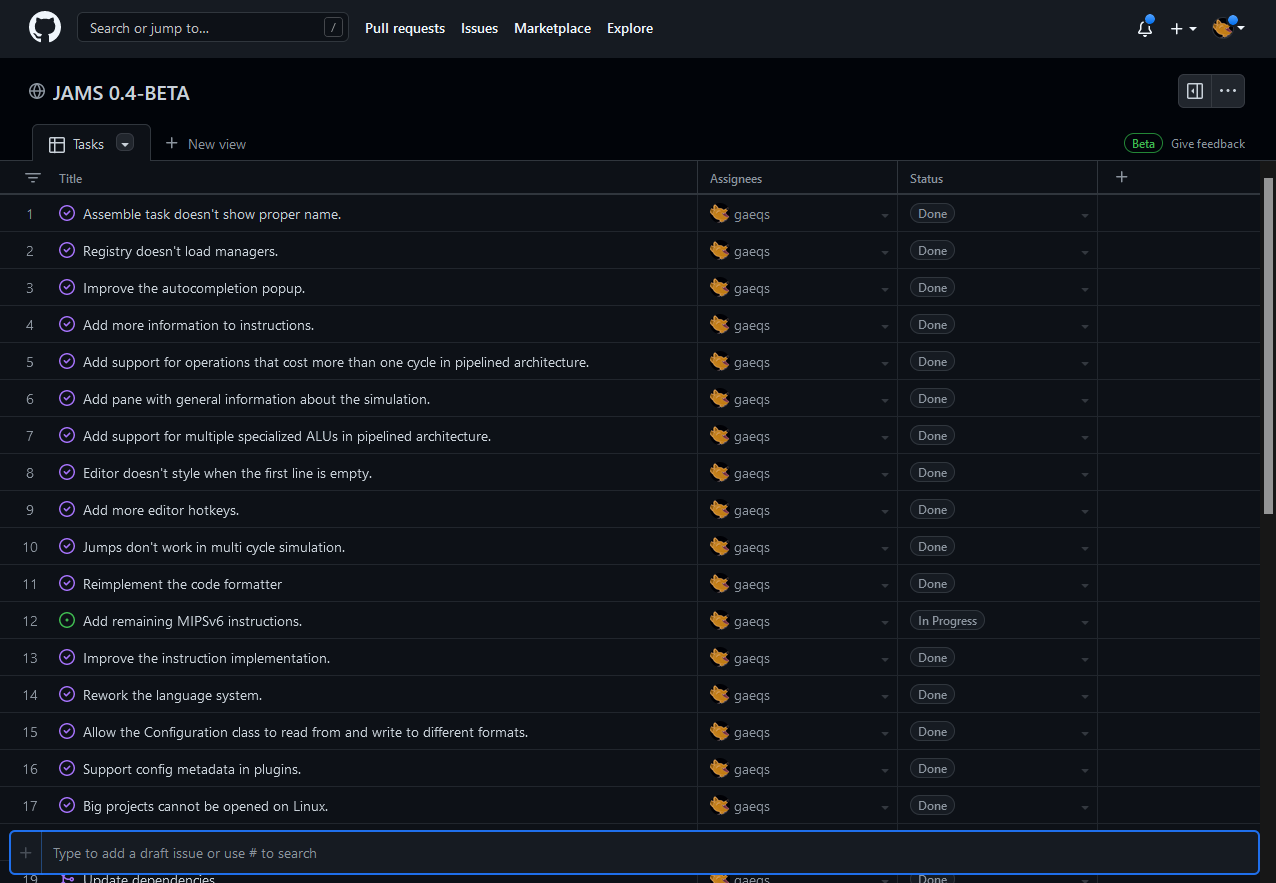
\includegraphics[width=\textwidth]{images/introduction/github}
    \caption{Proyecto de \textit{GitHub} para la versión 0.4-BETA}
    \label{fig:introduccion-github}
\end{figure}

    \chapter{Antecedentes}\label{ch:antecedentes}


\section{Antecedentes en los entornos de desarrollo \textit{MIPS}}
\label{sec:antecedentes-en-los-entornos-de-desarrollo-mips}

Los entornos de desarrollo \textit{MIPS} han estado presentes en
el mercado desde el principio de los años 90, quedando su desarrollo
estancado en la década de\delODR{l} 2010.
Estos entornos de desarrollo suelen estar enfocados al ámbito
educativo, con implementaciones muy básicas de la arquitectura.

A continuación se presentarán los principales
entornos de desarrollo y simuladores \textit{MIPS}:
\begin{itemize}
    \item \textbf{SPIM}\cite{SPIM}: es uno de los primeros simuladores
    \textit{MIPS32}, y uno de los más influyentes.
    La aplicación cuenta con un ensamblador que soporta las
    instrucciones más básicas de las primeras revisiones de la arquitectura.
    Es una aplicación que \textbf{se controla principalmente por consola},
    aunque las últimas versiones incorporan una interfaz gráfica
    desarrollada con el \textit{framework Qt}\cite{QT}.
    Los simuladores posteriores \textbf{tomarían mucha inspiración} de \textit{SPIM},
    implementando las llamadas al sistema desarrolladas específicamente
    para este simulador.
    \item \textbf{MARS}\cite{MARS}: desarrollado en la Universidad
    del estado de Missouri en 2005, \textit{MARS} es uno de los
    entornos de desarrollo \textit{MIPS32} más populares en el ámbito educativo.
    La aplicación, desarrollada en \textit{Java}\cite{JAVA}
    usando la librería \textit{Swing}\cite{SWING},
    presenta un editor de texto básico con \textbf{autocompletador}, un
    ensamblador con soporte para una gran variedad de instrucciones y
    pseudo-instrucciones y un simulador básico con diferentes herramientas
    desplegables.
    \item \textbf{WinMIPS64}\cite{WINMIPS64}: simulador
    de la arquitectura \textit{MIPS64} que implementa
    un procesador segmentado donde las instrucciones
    pueden tardar varios ciclos en ejecutarse.
    La herramienta más interesante de la aplicación
    es su \textbf{visualizador de flujo}.
    Existe un clon llamado \textit{EduMIPS64} desarrollado
    en \textit{Java} y multiplataforma.
    \item \textbf{Simula3MS}\cite{SIMULA3MS}: desarrollado en
    la Universidad de A Coruña, \textit{Simula3MS} es un
    pequeño entorno de desarrollo para \textit{MIPS32}
    con un simulador que permite \textbf{ejecutar el código en
    diferentes tipos de procesadores}.
    Está desarrollado en \textit{Java} con la librería \textit{Swing}.
    \item \textbf{DrMIPS}\cite{DRMIPS}: presenta un
    editor de texto, un ensamblador y un simulador
    para \textit{MIPS32}.
    La aplicación tiene un enfoque educativo, teniendo el simulador
    un \textbf{visualizador de los caminos del procesador}.
    \item \textbf{VisualMIPS32}\cite{VISUALMIPS32}: entorno
    de desarrollo \textit{MIPS32} desarrollado y
    utilizado por la Universidad de Sevilla para la enseñanza.
    Cuenta con un editor, un ensamblador y un simulador.
    Igual que \textit{WinMIPS64}, cuenta con un visualizador
    de flujo integrado.
\end{itemize}


\section{Antecedentes en los entornos de desarrollo}
\label{sec:antecedentes-en-los-entornos-de-desarrollo}

\textit{JAMS} también está fuertemente inspirado en los
entornos de desarrollo de carácter general más modernos.
Estas aplicaciones presentan una serie de funcionalidades que
caracterizan a los \textit{IDEs} de hoy en día:

\begin{itemize}
    \item \textbf{Nodos}: también conocidos como \textit{Widgets} o \textit{Tools}.
    Consisten en pequeñas herramientas que complementan al entorno.
    Antiguamente, estas herramientas solían desplegarse en una ventana diferente,
    siendo necesario seleccionarlas desde un menú desplegable en la ventana principal.
    Actualmente, los nodos suelen estar integrados \newODR{a} los lados de la ventana principal,
    siendo estos capaces de ser desplegados pulsando un botón en las barras laterales
    de la aplicación.
    Estos nodos son altamente personalizables, pudiendo el usuario cambiar su posición
    y el modo de despliegue.
    \item \textbf{Proyectos}: los entornos de desarrollo modernos están estructurados
    alrededor del concepto de proyecto.
    Un proyecto es un conjunto de archivos que componen el código fuente de una aplicación.
    Actualmente, no existe ningún entorno de desarrollo especializado en \textit{MIPS32}
    que presente esta característica.
\end{itemize}

Actualmente, existe una gran cantidad de entornos de desarrollo en el mercado:
específicos y generales, complejos y ligeros.
Cada uno de ellos presenta unas características diferentes que los hace único.

A continuación se presentarán algunos de los principales
entornos de desarrollo:
\begin{itemize}
    \item \textbf{Microsoft Visual Studio}\cite{VISUALSTUDIO}: entorno de desarrollo
    integrado general y complejo desarrollado por \textit{Microsoft}.
    Está programado en C++ y C\#, con soporte para componentes.
    Estos componentes son los que permiten añadir soporte para diversas tecnologías
    al entorno de desarrollo, ya que de por sí tiene soporte para una pequeña
    variedad de tecnologías.
    Junto a \textit{Intellij IDEA}, \textit{Microsoft Visual Studio} ha sido uno
    de los pioneros en integrar sus herramientas a la ventana principal.
    \textit{Microsoft Visual Studio} está disponible en tres versiones: la versión
    \textit{Community} para uso no comercial, la versión \textit{Professional} para
    proyectos comerciales y la versión \textit{Enterprise}, siendo esta la versión
    con más características.
    Las tres versiones son de \textbf{código privativo}.
    \item \textbf{Visual Studio Code}\cite{VISUALSTUDIOCODE}:
    es la alternativa de código abierto de \textit{Microsoft}.
    \textit{Visual Studio Code} es un entorno de desarrollo general
    y ligero \textit{desarrollado en HTML/CSS/TS} que sigue la misma filosofía
    de componentes de \textit{Microsoft Visual Studio}.
    \item \textbf{Eclipse}\cite{ECLIPSE}: creado por \textit{IBM} y actualmente
    desarrollado por \textit{Eclipse Foundation}.
    \textit{Eclipse} es entorno de desarrollo complejo desarrollado en \textit{Java},
    centrándose principalmente en el \textbf{desarrollo de aplicaciones para dicho lenguaje}.
    Actualmente, \textit{Eclipse} se ha convertido en un \textit{IDE} general que
    permite desarrollar en más de 20 lenguajes de programación.
    \textit{Eclipse} es de código abierto y totalmente gratis.
    \item \textbf{Intellij IDEA / \textit{IDEs} de \textit{JetBrains}}\cite{INTELLIJIDEA}:
    \textit{JetBrains} sigue una filosofía diferente al introducir
    soporte a un nuevo lenguaje de programación.
    Al principio, lanzan un componente para todos sus entornos de desarrollo,
    el cual da la habilidad de desarrollar en una nueva tecnología.
    Una vez el componente es lo suficientemente maduro, \textit{JetBrains}
    \textbf{lanza un nuevo entorno de desarrollo} para el lenguaje de programación
    en concreto.
    Todos estos entornos de desarrollo tienen la misma base, creada a
    principios de los años 2000 para \textit{Intellij IDEA}, su primer \textit{IDE}.
    Salvo algunas excepciones, todos los entornos de desarollo de \textit{JetBrains}
    son de código privativo y de pago, necesitando una licencia para poder usarlos.
    Las únicas excepciones son las versiones \textit{Community} de \textit{Intellij IDEA}
    y \textit{PyCharm}, de código abierto y para uso no comercial.
\end{itemize}

    \chapter{Tecnologías base del proyecto}\label{ch:tecnologias-base-del-proyecto}

En este capítulo se abordará la búsqueda, investigación y creación de las tecnologías
básicas necesarias para el desarrollo de \textit{JAMS}, empezando por la búsqueda
de un lenguaje de programación y \textit{framework} de aplicaciones gráficas adecuados
para el proyecto, y terminando definiendo los componentes más básicos desarrollados
para el entorno base.

\section{Definición de los requisitos de las tecnologías candidatas}
\label{sec:definicion-requisitos-tecnologías-candidatas}

Actualmente, existe una gran variedad de librerías y \textit{frameworks} gráficos que permiten
crear aplicaciones de una manera rápida y sencilla.
Estas tecnologías se pueden clasificar dependiendo de una gran cantidad de criterios.

Según su nivel de abstracción:
\begin{itemize}
    \item \textbf{Librerías de bajo nivel:} son más cercanas al \textit{hardware} gráfico.
    Permiten tener un gran control sobre los gráficos, pero no son adecuadas para
    interfaces gráficas de usuarios.
    Algunos ejemplos de librerías de bajo nivel son \textit{OpenGL}\cite{OPENGL},
    \textit{Vulkan}\cite{VULKAN} o \textit{DirectX}\cite{DIRECTX}.
    \item \textbf{Librerías de alto nivel}: incorporan una capa de abstracción sobre el \textit{hardware} gráfico.
    Permiten generar interfaces gráficas de usuario mediante una arquitectura ya definida.
    Algunos ejemplos de librerías de alto nivel son \textit{Qt}\cite{QT},
    \textit{JavaFX}\cite{JAVAFX}, \textit{Swing}\cite{SWING}, \textit{GTK} o
    \textit{Compose Multiplatform}\cite{COMPOSE}.
\end{itemize}

Según su disponibilidad en varias plataformas:
\begin{itemize}
    \item \textbf{Librerías exclusivas:} son librerías que solo están disponibles en una plataforma.
    Algunos ejemplos de librerías exclusivas son \textit{Windows Forms}\cite{WINDOWSFORMS}
    y \textit{DirectX} en \textit{Windows},
    \textit{Metal} y \textit{QuickDraw} en \textit{MacOS}
    o \textit{AndroidX/Graphics} y \textit{Jetpack Compose}\cite{COMPOSE}
    en \textit{Android}.
    \item \textbf{Librerías multiplataforma:} están disponibles en una gran variedad de plataformas.
    Algunos ejemplos de librerías multiplataforma son \textit{Qt}, \textit{JavaFX}, \textit{Swing}, \textit{GTK}
    o \textit{Compose Multiplatform}.
\end{itemize}

Un aspecto muy importante al elegir candidatos es el \textbf{lenguaje de programación}
en el que las librerías están disponibles.
Las librerías de bajo nivel suelen estar disponibles en una gran variedad de lenguajes, mientras que las
librerías de alto nivel suelen incorporar paradigmas propios del lenguaje de programación en el que están
desarrolladas.

Para el desarrollo de la aplicación se desea utilizar una librería gráfica \textbf{moderna},
\textbf{de alto nivel}, \textbf{multiplataforma}, disponible en un lenguaje de programación estable,
con una comunidad grande y \textbf{rápido tanto en el desarrollo como en la ejecución}.
Otro requisito crucial es que el lenguaje permita \textbf{vincular código externo} de manera
sencilla y en \textbf{tiempo de ejecución}.

Estos requisitos reduce la lista de tecnologías en los siguientes candidatos:
\begin{itemize}
    \item \textbf{HTML, CSS y TypeScript:} este conjunto de tecnologías es muy popular actualmente
    para la creación de aplicaciones web y de escritorio. \textit{IDEs} muy famosos como
    \textit{Visual Studio Code} están desarrollados con estas tecnologías.
    \item \textbf{Kotlin / Compose Multiplatform:} \textit{Compose Multiplatform} es una librería gráfica
    para \textit{Kotlin}, un lenguaje de programación muy joven y potente que tiene el respaldo de
    grandes compañías como \textit{JetBrains} y \textit{Google}.
    \item \textbf{Java/ JavaFX:}
    \textit{JavaFX} puede considerarse la evolución natural de \textit{Swing},
    la herramienta principal para el desarrollo de aplicaciones gráficas basadas en \textit{Java}.
    \textit{JavaFX} es una librería moderna y rápida que, gracias a que está desarrollada en \textit{Java},
    puede ser empleada por otros lenguajes de programación que corren sobre la \textit{JVM}
    \footnote{\textit{Java Virtual Machine}}, como es el caso de \textit{Scala}, \textit{Groovy} o el ya mencionado
    \textit{Kotlin}.
\end{itemize}

El trío \textit{HTML / CSS / TypeScript} suele ser una buena elección para editores y otras
aplicaciones ligeras, pero la falta de velocidad en la ejecución y la falta de consistencia por estar
basado \textit{TypeScript} en \textit{JavaScript} descarta esta opción por parte del simulador.

\textit{Kotlin / Compose Multiplatform} es una elección muy sólida actualmente, pero esta
tecnología seguía en fase \textit{beta} cuando este proyecto empezó, por lo que también ha quedado
descartada.

Finalmente, \textbf{se ha optado por utilizar el par de tecnologías \textit{Java / JavaFX}}
para el desarrollo de la aplicación, ya que cumple con todos los requisitos: \textit{Java} es un
lenguaje de programación muy estable, multiplataforma y rápido tanto en la ejecución como en
el desarrollo.
También es el lenguaje de programación con la comunidad de desarrolladores más grande.
\textit{JavaFX} es una alternativa moderna a \textit{Swing} que permite desarrollar aplicaciones
fácilmente personalizables que se alejan del ya conocido estilo de interfaz \textit{Java}.

Centrándose en otras tecnologías necesarias, se ha utilizado el entorno de desarrollo
\textit{Intellij IDEA}\cite{INTELLIJIDEA} y el sistema de
automatización \textit{Gradle} para la construcción del proyecto.

\subsection{En defensa de \textit{Java}}\label{subsec:en-defensa-de-java}

Muchos desarrolladores piensan que \textit{Java} es un lenguaje de programación verboso, lento, pesado
y con el único propósito de crear aplicaciones \textit{Spring}.
Que la mayoría de aplicaciones \textit{Java} estén desarrolladas en versiones \textit{vanilla}
\footnote{Estándar, sin modificar} de \textit{Swing} y en versiones de \textit{Java} de hace más
de un lustro no ayuda en su reputación.

La realidad es muy diferente: su equipo de desarrollo lleva años reinventando su tecnología,
con nuevas características que acercan a \textit{Java} a lenguajes de programación mucho más modernos.
La velocidad de ejecución también se ha incrementado considerablemente, posicionándose en uno de los
lenguajes de programación que más rápido ejecutan.

Un gran ejemplo del drástico cambio que ha sufrido \textit{Java} en los últimos años son los
\textit{records}: clases de datos que son inmutables.

\begin{lstlisting}[language=Java,style=java,frame=single,label={lst:java-comparacion-18}]
public record Cat(String name, UUID owner) {
}
\end{lstlisting}

El código equivalente en \textit{Java} 8 sería el siguiente:

\begin{lstlisting}[language=Java,style=java,frame=single,label={lst:java-comparacion-8}]
public final class Cat {
    private final String name;
    private final UUID owner;

    public Cat(String name, UUID owner) {
        this.name = name;
        this.owner = owner;
    }

    public String name() { return name; }

    public UUID owner() { return owner; }

    @Override
    public boolean equals(Object obj) {
        if (obj == this) return true;
        if (obj == null || obj.getClass() != this.getClass())
            return false;
        var that = (Cat) obj;
        return Objects.equals(this.name, that.name) &&
                Objects.equals(this.owner, that.owner);
    }

    @Override
    public int hashCode() { return Objects.hash(name, owner); }

    @Override
    public String toString() { return "Cat[" + "name=" + name
        + ", " + "owner=" + owner + ']'; }

}
\end{lstlisting}

La nueva arquitectura basada en módulos que presenta las librerías de \textit{Java}
ayuda mucho en la distribución de aplicaciones de escritorio, pudiendo generar un instalador
convencional que instala la aplicación junto con una versión local de la \textit{JVM} que no
suele superar los 30 MB\cite{JPACKAGE}.
Gracias a este sistema de distribución, la aplicación podrá contar con versiones
de \textit{Java} actuales sin que los usuarios tengan que pasar por complejas instalaciones.

Como dato final, existen muchas aplicaciones que se ejecutan sobre la \textit{JVM}
sin que el usuario se de cuenta.
Este es el caso de todos los \textit{IDEs} desarrollados por \textit{JetBrains}, los cuales
usan la librería \textit{Swing} con un estilo avanzado, como se puede observar en la figura
\ref{fig:java-intellij-idea}.

\begin{figure}[h]
    \centering
    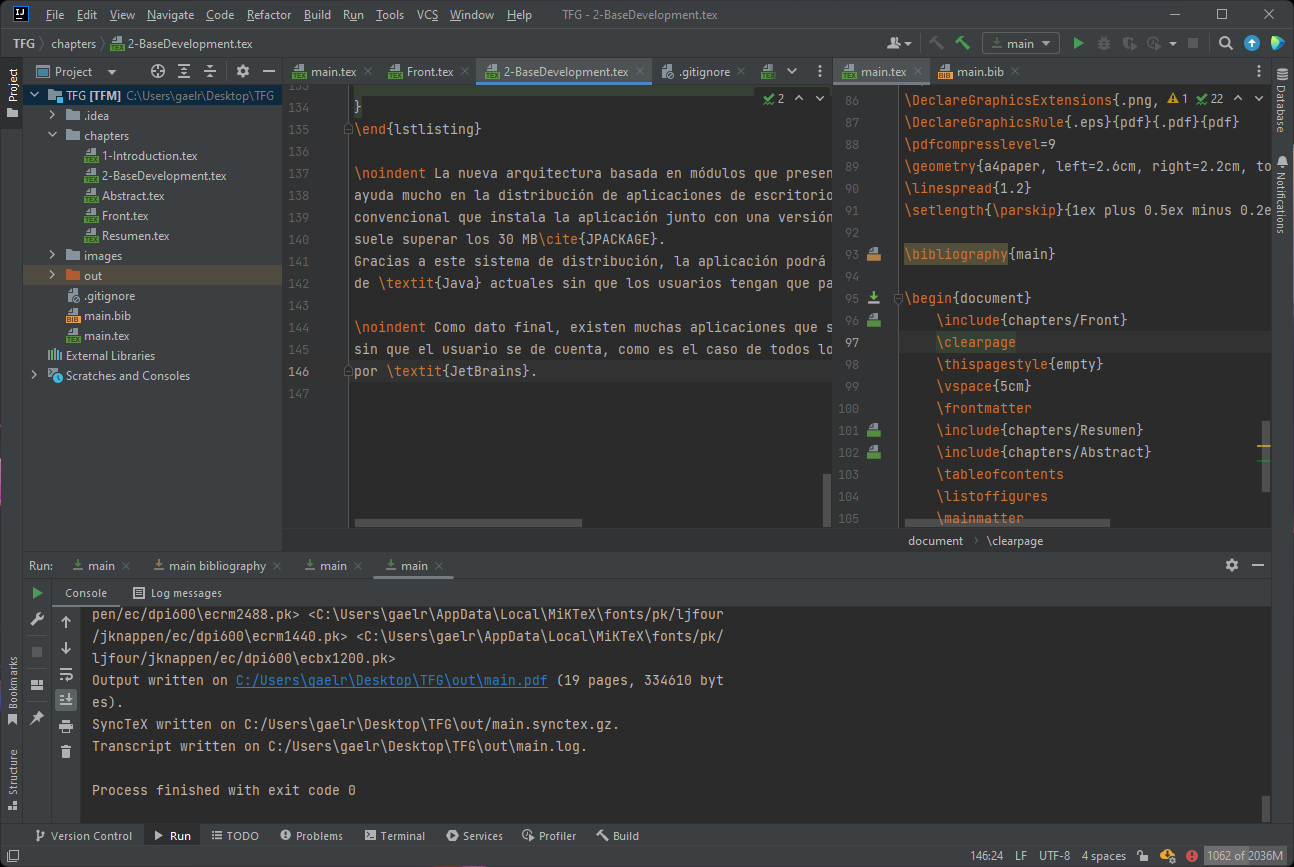
\includegraphics[width=\textwidth]{images/base/intellij-idea}
    \caption{\textit{Intellij IDEA}}
    \label{fig:java-intellij-idea}
\end{figure}


\section{Estructura del proyecto}\label{sec:estructura-del-proyecto}

\textit{JAMS} sigue los estándares de estructura de \textit{Gradle}\cite{GRADLE_ORGANIZING}.
Esto hace que su estructura sea muy similar a otras aplicaciones que usan el mismo
sistema de automatización.

\subsection{Tareas}\label{subsec:tareas}

El elemento más importante del directorio raíz es el archivo \textbf{build.gradle}.
En él se especifican las dependencias y se define cómo el proyecto debe ser compilado.
Las \textbf{tareas} son las encargadas de definir dicho comportamiento.

Las dos tareas más importantes son las siguientes:
\begin{itemize}
    \item \textbf{jpackage:} permite generar un instalador de la aplicación específico
    para la máquina que ejecuta la tarea.
    \item \textbf{bundle:} genera un archivo \textit{jar} con la aplicación y todas
    sus dependencias.
    Este archivo puede ser ejecutado en cualquier sistema operativo que pueda correr
    \textit{Java} y esté soportado por \textit{JavaFX}.
\end{itemize}

Para ejecutar estas tareas ha de usarse el \textit{script} $gradlew$.
Este comando descargará \textit{Gradle} si es necesario y ejecutará
la tarea pasada como argumento.
Todos estos comportamientos están automatizados en \textit{GitHub}
mediante los \textit{scripts} dentro de la carpeta $.github$.

\subsection{Módulos y paquetes}\label{subsec:modulos-y-paquetes}

Dentro de la carpeta $src$ están definidos los dos módulos principales del
proyecto: $main$ y $test$.

El módulo $main$ es el encargado de almacenar todo el código fuente
de la aplicación.
Puede ser considerado el módulo más importante de todo el proyecto.
El módulo $test$ define todas las pruebas unitarias que el módulo $main$
debe superar para que la aplicación se compile con éxito.

El código fuente almacenado en el módulo $main$ está separado en diferentes
paquetes \textit{Java}:
\begin{itemize}
    \item \textbf{collection:} contiene una serie de colecciones modificadas.
    \item \textbf{configuration:} contiene el sistema de configuraciones.
    \item \textbf{event:} contiene el sistema de eventos.
    \item \textbf{file:} contiene los tipos de archivo definidos en la aplicación.
    \item \textbf{gui:} contiene toda la interfaz de la aplicación.
    \item \textbf{language:} contiene el sistema de idiomas.
    \item \textbf{manager:} contiene el sistema de gestores.
    \item \textbf{mips:} contiene todas las herramientas relacionadas con la arquitectura \textit{MIPS32}.
    \item \textbf{plugin:} contiene el sistema de componentes.
    \item \textbf{project:} contiene el sistema de proyectos.
    \item \textbf{task:} contiene el sistema de hijos y tareas asíncronas.
    \item \textbf{utils:} contiene clases útiles utilizadas por los anteriores paquetes.
\end{itemize}


\section{Proyectos}\label{sec:interfaz-grafica}

\textit{JAMS} es un \textit{IDE} basado en \textbf{proyectos}.
Un proyecto está formado por una carpeta y las siguientes propiedades:
\begin{itemize}
    \item \textbf{Tipo de proyecto:} especifica el tipo de proyecto.
    En una versión sin componentes este valor solo puede tomar el valor \textit{MIPS}.
    \item \textbf{Propiedades del proyecto:} parámetros necesarios por el tipo de proyecto.
    Configuran aspectos concretos y generales de todo el proyecto.
    \item \textbf{Archivos a ensamblar:} lista de archivos que el ensamblador tendrá en cuenta
    al ensamblar el proyecto.
    \item \textbf{Configuraciones:} especifican propiedades \textbf{de una ejecución} del proyecto.
    Es decir, configuran el simulador.
    Un proyecto puede tener varias configuraciones, y el usuario ha de elegir una al crear una
    simulación.
\end{itemize}

Los proyectos son almacenados en carpetas.
Una carpeta de un proyecto tiene la siguiente estructura:

\begin{center}
    \basictree{
        [MyProject
        [.jams
        [data.json]
        [files\_to\_assemble.json]
        ]
        [Simulation Files
        [MySimulationFile.txt]
        ]
        [MyAsmFile.asm]
        ]
    }
\end{center}

Cada proyecto tiene dos carpetas por defecto: \textbf{.jams} y
\textbf{Simulation Files}.
La carpeta \textbf{.jams} contiene los datos del proyecto que \textit{JAMS}
gestiona de manera automática.
Esta carpeta está oculta y no debe ser modificada por el usuario.
El archivo \textbf{data.json} contiene el tipo de proyecto y sus propiedades,
mientras que \textit{files\_to\_assemble.json} contiene la listas de archivos
que el ensamblador ha de usar.
La carpeta \textit{Simulation Files} actúa de carpeta raíz del simulador:
todos los archivos que escriba o lea el simulador deben estar situados dentro
de esta carpeta.
    \chapter{Desarrollo del entorno base}\label{ch:desarrollo-del-entorno-base}


\section{Interfaz de usuario}\label{sec:interfaz-de-usuario}

La interfaz de \textit{JAMS} es muy similar a las interfaces que presentan los \textit{IDEs} modernos.
Todas las herramientas están encapsuladas en $nodos$.
Cada nodo se puede desplegar en los laterales del editor.
Más concretamente, se pueden desplegar dos nodos por cada lado del editor.

\begin{figure}[H]
    \centering
    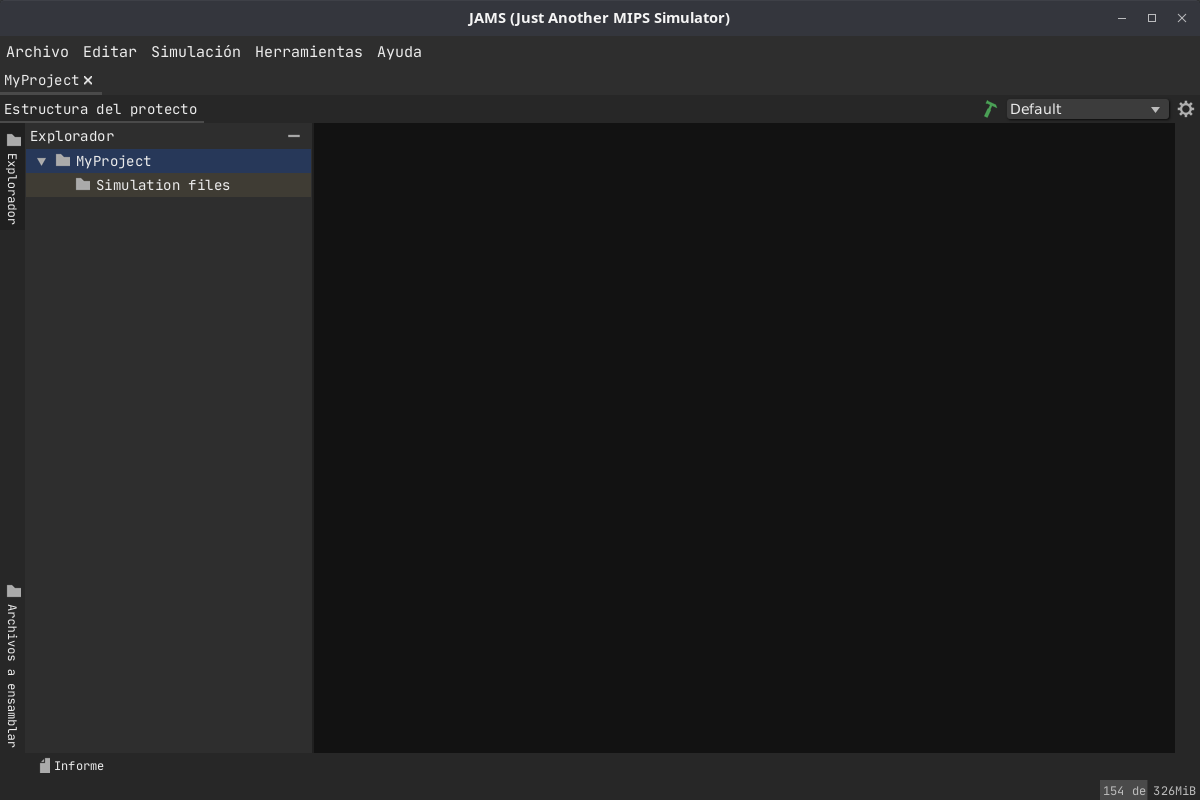
\includegraphics[width=0.8\textwidth]{images/base/jams-basic}
    \caption{\textit{Editor de \textit{JAMS} en su forma más básica}}
    \label{fig:jams-basic}
\end{figure}

\noindent Los nodos también se pueden configurar para que se desplieguen
en una ventana aparte.
Esto permite poder desplegar un número indefinido de nodos al mismo tiempo.
El modo de despliegue se puede configurar presionando el botón secundario sobre
el botón del nodo.

\begin{figure}[H]
    \centering
    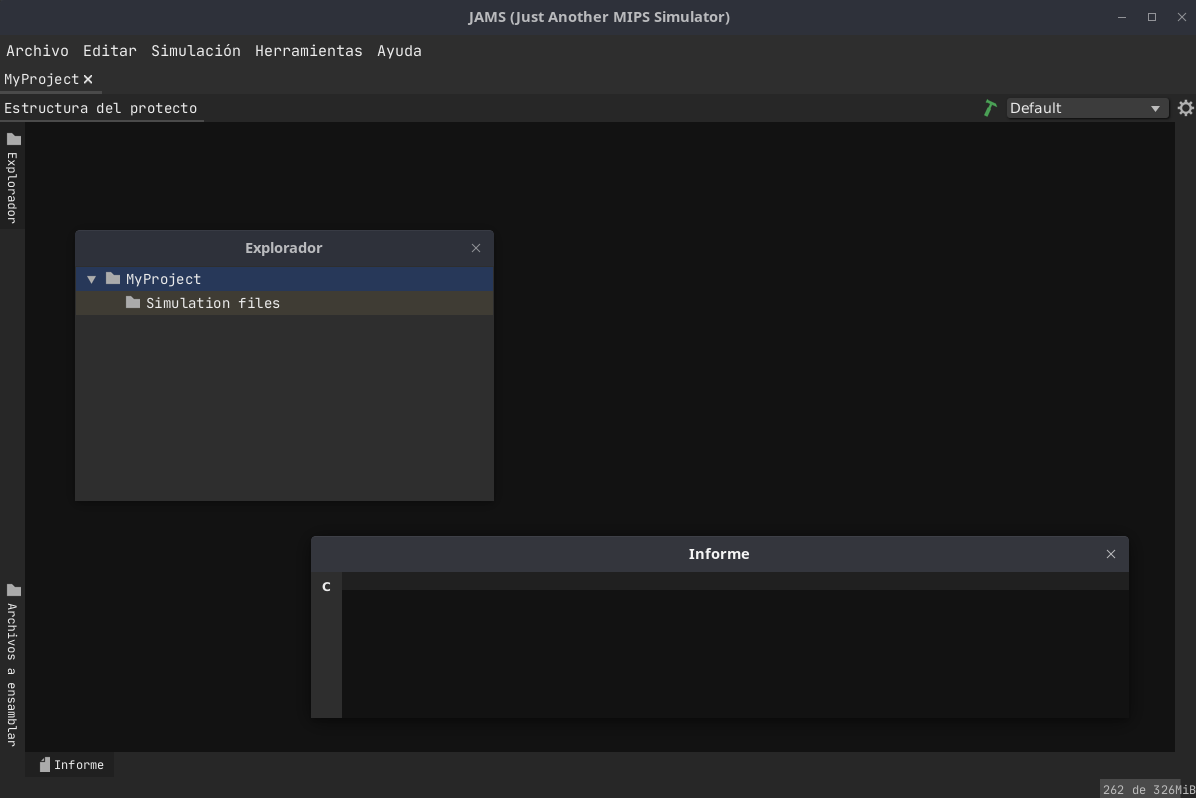
\includegraphics[width=0.8\textwidth]{images/base/jams-windows}
    \caption{\textit{Editor de \textit{JAMS} con ventanas desplegadas}}
    \label{fig:jams-windows}
\end{figure}

\subsection{Menú superior}\label{subsec:menu-superior}

El menú superior de \textit{JAMS} funciona de manera idéntica
a cualquier otro programa.
Por defecto existen cinco secciones:
\begin{itemize}
    \item \textbf{Archivo}: permite crear o abrir nuevos proyectos, además de
    acceder a la configuración.
    \item \textbf{Editar:} permite acceder a los comandos del editor de texto.
    \item \textbf{Simulación:} permite acceder a los comandos de simulación.
    \item \textbf{Herramientas:} permite habilitar o deshabilitar nodos.
    \item \textbf{Ayuda:} permite acceder a ayuda sobre \textit{JAMS}.
\end{itemize}

\subsection{Proyectos abiertos}\label{subsec:proyectos-abiertos}

Los proyectos abiertos aparecen justo debajo del menú superior.
Cada proyecto está representado por una pestaña, lo que facilita alternar entre
proyectos abiertos.
Si se cierran todos los proyectos, \textit{JAMS} cerrará el editor y trasladará
al usuario a la ventana de inicio.

\noindent Los proyectos presentan una lista de pestañas con todas las secciones
que tienen abiertas.
Normalmente, la primera pestaña representa el editor del proyecto, mientras que
las siguientes representan las simulaciones que el usuario vaya creando.

\begin{figure}[H]
    \centering
    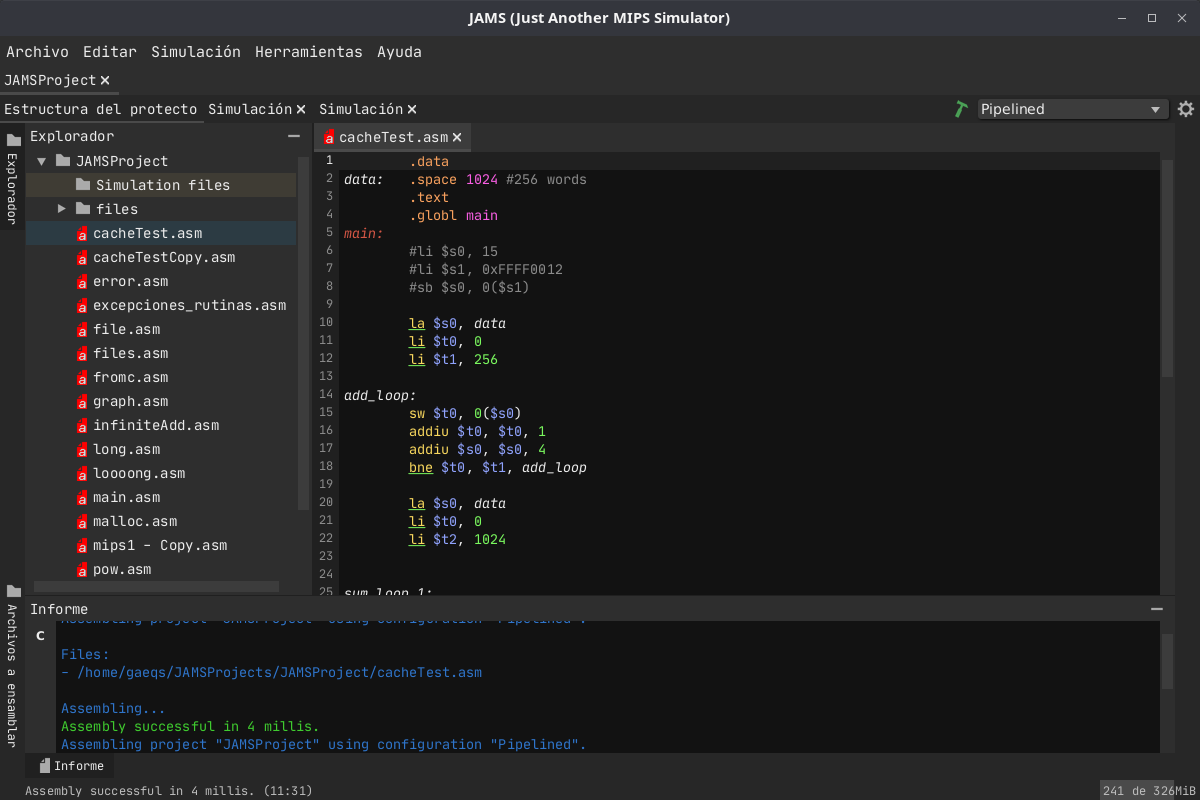
\includegraphics[width=0.8\textwidth]{images/base/jams-sections}
    \caption{\textit{Editor de \textit{JAMS} con varias simulaciones creadas}}
    \label{fig:jams-sections}
\end{figure}

\noindent Cada sección tiene una \textbf{barra de herramientas} propia.
Esta barra está situada a la izquierda de la lista de secciones, y permite
ejecutar acciones relacionadas con la sección actual.

\subsection{Barra inferior}\label{subsec:barra-inferior}

La barra inferior del editor es común a todas las secciones.
En esta, se informa del último mensaje escrito en el \textbf{informe}.
A la izquierda también se muestra la memoria que está usando actualmente
\textit{JAMS}.
Al estar creada la aplicación en \textit{Java}, esta utiliza un recolector
de basura.
Se puede forzar el paso del recolector de basura pulsando el panel que informa
sobre el uso de memoria.

\subsection{Ventana principal}\label{subsec:ventana-principal}

Si \textit{JAMS} no tiene ningún proyecto que mostrar, se mostrará la ventana
principal.
En esta ventana se pueden encontrar cuatro apartados:
\begin{itemize}
    \item \textbf{Proyectos:} en este apartado se encuentran los proyectos más
    recientes.
    También se puede abrir un proyecto ya existente.
    \item \textbf{Nuevo proyecto:} este apartado permite crear nuevos proyectos.
    Un componente puede añadir su propio creador de proyectos.
    \item \textbf{Configuración:} muestra la ventana de configuración.
    Permite configurar \textit{JAMS} antes de abrir un proyecto.
    \item \textbf{Acerca de:} muestra información básica sobre \textit{JAMS}.
\end{itemize}

\begin{figure}[H]
    \centering
    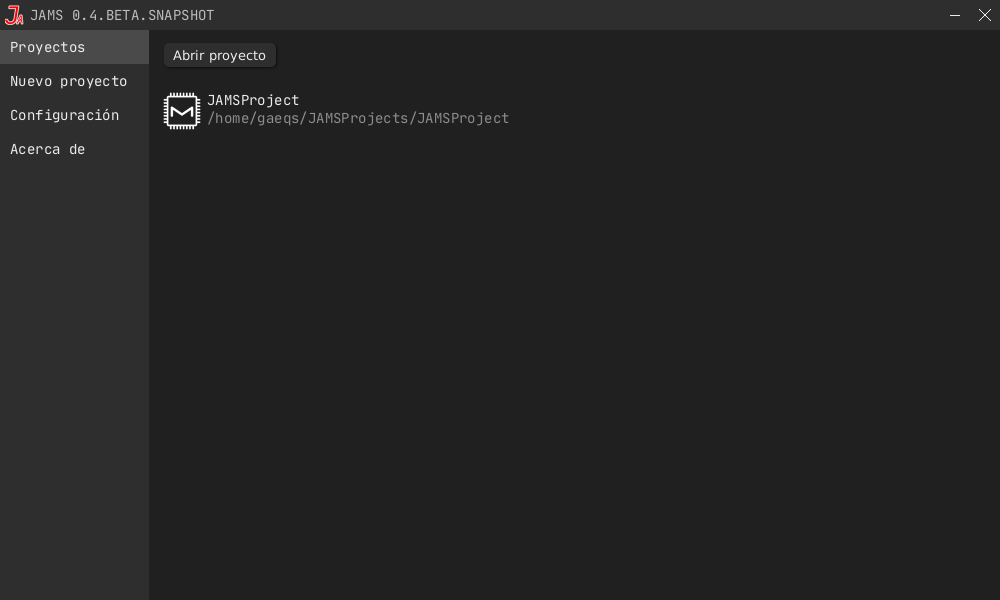
\includegraphics[width=0.8\textwidth]{images/base/jams-main-projects}
    \caption{\textit{Ventana principal mostrando los proyectos recientes}}
    \label{fig:jams-main-projects}
\end{figure}

\begin{figure}[H]
    \centering
    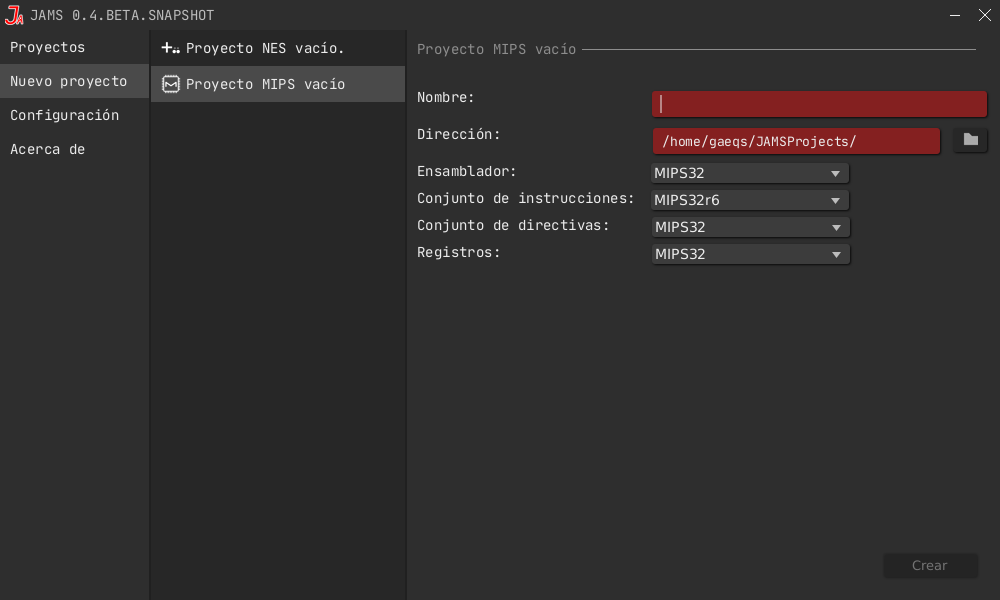
\includegraphics[width=0.8\textwidth]{images/base/jams-main-new-project}
    \caption{\textit{Ventana de creación de nuevos proyectos}}
    \label{fig:jams-main-new-project}
\end{figure}


\section{Idiomas}\label{sec:idiomas}

Igual que cualquier aplicación moderna, \textit{JAMS} presenta un sistema de
localización basado en paquetes de idiomas.
Cualquier usuario o componente puede crear un paquete que añada
o modifique un idioma.
El sistema de idiomas utiliza el estándar \textit{Unicode}, lo que permite
a los idiomas usar caracteres especiales en sus mensajes.

\subsection{Estructura de un paquete}\label{subsec:estructura-de-un-paquete}

Un paquete de idiomas es una carpeta o un archivo comprimido
que contienen un archivo \textbf{language.json} y varios archivos \textit{YAML}.
Esta carpeta o archivo estará situado dentro de un componente
o dentro de la carpeta \textbf{\textasciitilde/JAMS/languages}.
Un ejemplo de un archivo \textbf{language.json} sería el siguiente:

\begin{lstlisting}[frame=single,label={lst:language.json}]
{
  "name": "English",
  "priority": 0,
  "files": [
    "actions.yml",
    "configuration.yml",
    "directives.yml"
  ]
}
\end{lstlisting}

\noindent Dentro de este archivo se encuentran los siguientes parámetros:
\begin{itemize}
    \item \textbf{name:} es el nombre del idioma.
    Este nombre es el que será mostrado al usuario
    y actúa como identificador del idioma.
    \item \textbf{files:} son los archivos \textit{YAML} que componen el paquete.
    \item \textbf{priority:} es la prioridad del paquete si existen varios
    paquetes para el mismo idioma.
    Cuanto más alto sea el número, más prioridad tiene el paquete.
    Esta propiedad es opcional y por defecto toma el valor 0.
\end{itemize}

\noindent Los archivos \textit{YAML} pueden estar en carpetas dentro del paquete,
y deben estar definidos en el archivo \textbf{language.json} con una
dirección relativa a la raíz del paquete.
Un ejemplo de archivo \textit{YAML} sería el siguiente:

\begin{lstlisting}[frame=single,label={lst:interface.yml}]
START_TITLE: JAMS {VERSION}
START_PROJECTS: Projects
START_NEW_PROJECT: New project
START_ABOUT: About
BOTTOM_BAR_MEMORY: '{USED} of {TOTAL}MiB'
BOTTOM_BAR_MEMORY_TOOLTIP: Click to execute the garbage collector.
\end{lstlisting}

\subsection{Extensiones}\label{subsec:idiomas-extensiones}

Puede existir el caso donde varios paquetes hagan referencia al mismo idioma.
Este problema de colisión se soluciona gracias a las extensiones.
Un paquete actúa siempre como una extensión de un idioma.
Esta extensión tiene una prioridad que se define en el archivo
\textbf{language.json} del paquete.
Si dos extensiones tienen la misma prioridad, el orden se resuelve
por orden de creación de la extensión, siendo el último en ser creado
el que tenga más prioridad.
El mensaje ligado a un identificador será el de la extensión con más prioridad
que contenga un mensaje ligado al identificador.
Gracias a este pequeño sistema de extensiones, los usuarios podrán crear modificaciones
y los componentes podrán añadir nuevos mensajes.

\subsection{Instalación y selección de un idioma}\label{subsec:instalacion-y-seleccion-de-un-idioma}

Los usuarios pueden instalar un paquete de idioma arrastrando la carpeta o
archivo comprimido que lo contiene dentro de la carpeta \textbf{\textasciitilde/JAMS/languages}.
Una vez hecho esto, \textit{JAMS} mostrará los cambios realizados por el paquete
de idioma.
Si el paquete de idioma contiene un idioma nuevo, el usuario podrá seleccionarlo
desde la configuración.

\noindent \textit{JAMS} necesita que dos idiomas estén seleccionados al mismo tiempo:
el \textbf{idioma a mostrar} y el \textbf{idioma de respaldo}.
El idioma de respaldo se usará cuando el idioma a mostrar no defina un mensaje
necesario por la aplicación.
El usuario puede cambiar tanto el idioma a mostrar como el idioma de respaldo.
Cuando un idiomas es eliminado y este está seleccionado, \textit{JAMS}
buscará el idioma más adecuado para reemplazarlo.

\noindent El cambio de idioma, al igual que el resto de los parámetros de configuración,
tienen un efecto \textbf{instantáneo} en la aplicación, por lo que no es necesario
reiniciar la aplicación para que el cambio de idioma tenga efecto.


\section{Temas}\label{sec:temas}

Los temas de JAMS funcionan de la misma manera que el estilo de una página web:
mediante archivos \textit{CSS}.
funcionamiento de los temas es muy similar al funcionamiento de los idiomas:
los temas son empaquetados en una carpeta o archivo comprimido,
con un archivo \textit{JSON} que actúa como punto de entrada (\textbf{theme.json})
y un conjunto de archivos \textit{CSS}.

\noindent A diferencia de los idiomas, un desarrollador que implemente nuevos
nodos a la escena de \textit{JAMS} no require gestionar ningún aspecto
de los temas: el tema que el usuario tenga seleccionado será implementado
de manera transparente gracias al sistema de temas de \textit{JavaFX}.

\subsection{Estructura}\label{subsec:estructura}

El archivo \textbf{theme.json} define el nombre y los archivos
\textit{CSS} incluidos en el tema.
Un ejemplo de archivo theme.json sería el siguiente:
\begin{lstlisting}[frame=single,label={lst:theme.json}]
{
  "name": "Light Theme",
  "dependencies": ["Other Theme"],
  "files": [
    "extra.css"
  ]
}
\end{lstlisting}

\noindent Un archivo \textbf{theme.json} presenta los siguientes parámetros:
\begin{itemize}
    \item \textbf{name:} es el nombre del tema.
    Este nombre es el que será mostrado al usuario
    y actúa como identificador del tema.
    \item \textbf{files:} son los archivos \textit{CSS} que componen el paquete.
    \item \textbf{dependencies:} los temas de los que este tema depende.
    El estilo de estos temas será añadido al estilo del tema definido.
    Este parámetro es opcional.
\end{itemize}

\noindent Estén definidos o no las dependencias,
todo tema depende del tema $Common$.
Este tema actúa de base, y define el estilo básico de \textit{JAMS}.
Este tema define muchas variables globales, pero no le asigna ningún
valor a ninguna de ellas.

\subsection{Variables globales}\label{subsec:variables-globales}

Las variables globales permiten definir el color de los diferentes
componentes de manera muy sencilla.
Un tema debe asignar un color a todas las variables del tema $Common$.
Esta tarea se debe hacer en el archivo especial \textbf{global.css}.
Este archivo es un archivo especial que siempre está incluido en el tema y,
al compilar, será envuelto en una sección global \textit{CSS} $*\{ \}$.
Esto permite que todos los componentes puedan usar
las variables asignadas en este archivo.
Un ejemplo de archivo \textbf{global.css} sería el siguiente:

\begin{lstlisting}[frame=single,label={lst:global.css}]
-theme-foreground: #222222;
-theme-foreground-darker: derive(-theme-foreground, 20%);
-theme-foreground-darker-2: derive(-theme-foreground, 40%);
-theme-foreground-lighter: #000000;
-theme-background: #f2f2f2;
-theme-background-darker: #e5e5e5;
-theme-background-darker-2: #eaeaea;
-theme-background-lighter: #f7f7f7;
-theme-background-pressed: derive(-theme-background, -10%);
-theme-background-darkest: #FFFFFF;
-theme-shadow: #555555;
-theme-header: #8faccc;
-theme-menu-item-hover: #4D6EAF;

...
\end{lstlisting}

\subsection{Extensiones}\label{subsec:temas-extensiones}

Igual que los idiomas, los temas funcionan mediante extensiones.
Todo paquete de temas es convertido en una extensión del tema que define.
Si existen varios paquetes apuntando al mismo tema, los dos coexistirán
como dos extensiones del mismo tema.
Una gran diferencia a los idiomas es que las extensiones de los temas
no tienen prioridad.
\textit{JavaFX} sigue el estándar
\textit{CSS}\footnote{\url{https://developer.mozilla.org/en-US/docs/Web/CSS/Specificity\#how_is_specificity_calculated}}
para la prioridad de las definiciones,
por lo que una capa de prioridades más es innecesaria.

\subsection{Instalación y selección de un tema}\label{subsec:instalacion-y-seleccion-de-un-tema}

\noindent Los usuarios pueden instalar un paquete de temas arrastrando la carpeta o
archivo comprimido que lo contiene dentro de la carpeta \textbf{\textasciitilde/JAMS/themes}.
Una vez hecho esto, \textit{JAMS} mostrará los cambios realizados por el paquete de temas.

\noindent Si el paquete contiene un tema nuevo, el usuario podrá seleccionarlo desde la configuración.
Cuando un tema es eliminado y este está seleccionado, \textit{JAMS}
buscará el tema más adecuado para reemplazarlo.

\noindent De la misma manera que en los idiomas, el cambio de tema tiene un
efecto \textbf{instantáneo} en la aplicación, por lo que no es necesario
reiniciar la aplicación pa que el cambio de tema tenga efecto.

\begin{figure}[H]
    \centering
    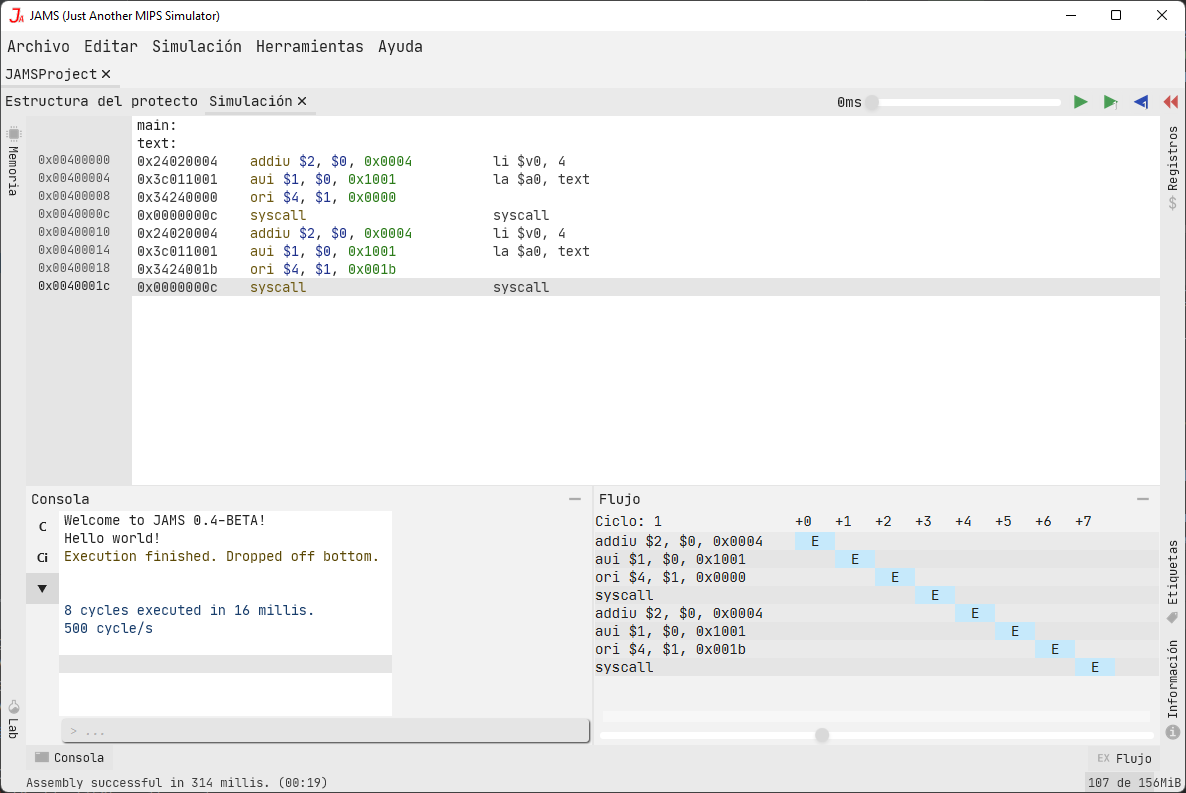
\includegraphics[width=0.8\textwidth]{images/base/jams-theme}
    \caption{\textit{JAMS} configurado para usar el modo claro}
    \label{fig:jams-light-theme}
\end{figure}


\section{Configuración}\label{sec:configuracion}

Igual que cualquier aplicación moderna, \textit{JAMS} presenta una
ventana de configuración donde el usuario podrá personalizar su experiencia.
Internamente, el sistema de configuraciones orbita alrededor de dos archivos \textit{JSON}:
\textbf{el archivo de valores} y el \textbf{archivo de estructura}.

\noindent El archivo de valores es el encargado de almacenar los valores de
todos los \textbf{nodos} de la configuración.
Existe dos versiones de este archivo:
el primero se encuentra en la carpeta \textbf{\textasciitilde/JAMS} y representa los \textbf{valores
actuales de la configuración}.
El segundo se encuentra dentro de la propia aplicación, y es el encargado de
proporcionar \textbf{los valores por defecto de cada nodo}.
Un componente podrá agregar nuevos valores a este archivo.

\begin{lstlisting}[frame=single,label={lst:main_config.json}]
{
    "language": {
        "default": "English",
        "selected": "English"
    }
}
\end{lstlisting}

\noindent El archivo de estructura o metadatos contiene información
relacionada sobre el propio nodo: el \textbf{tipo}, \textbf{región}
y \textbf{nombre} de cada nodo están definidos en este archivo.
Las secciones también tienen sus propios metadatos, especificando
el \textbf{nombre} de la sección y sus \textbf{regiones} con sus
\textbf{prioridades}.

\begin{lstlisting}[frame=single,label={lst:main_config_meta.json}]
{
    "language": {
        "meta": {
            "language_node": "CONFIG_LANGUAGE",
            "regions": {
                "language": 0
            }
        },
        "default": {
            "type": "language",
            "language_node": "CONFIG_LANGUAGE_DEFAULT",
            "region": "language"
        },
        "selected": {
            "type": "language",
            "language_node": "CONFIG_LANGUAGE_SELECTED",
            "region": "language"
        }
    }
}
\end{lstlisting}

\subsection{Interfaz de la configuración}\label{subsec:interfaz-de-la-configuración}

Para evitar que los usuarios tengan que modificar los valores de la configuración
externamente, se ha implementado una interfaz que permite modificar los
parámetros al vuelo dentro de la aplicación.
Esta interfaz es accesible directamente en la ventana de inicio o accediendo a ella
mediante la opción \textbf{Archivo > Configuración}.

\noindent Una vez la interfaz está abierta, el usuario encontrará dos nodos principales:
la lista de secciones y el visualizador de secciones.
La lista de secciones es un explorador que muestra todo el árbol de
secciones presente actualmente en la configuración.
Hay algunas secciones que contienen sub-secciones, las cuales se pueden
mostrar expandiendo la sección padre en la lista.
El visualizador de secciones muestra todos los parámetros de configuración
presentes en la sección seleccionada en la lista.
Esta interfaz aprovecha los metadatos proporcionados por el archivo
de estructura para proporcionar una interacción adecuada entre el usuario
y los diferentes parámetros.
La interfaz es extensible, pudiendo los componentes añadir nuevos tipos de datos.
La sección seleccionada puede tener un tipo de vista especial
que modifique el aspecto general del visualizador de secciones.
Es el caso de las secciones de componentes y de acciones.

\begin{figure}[H]
    \centering
    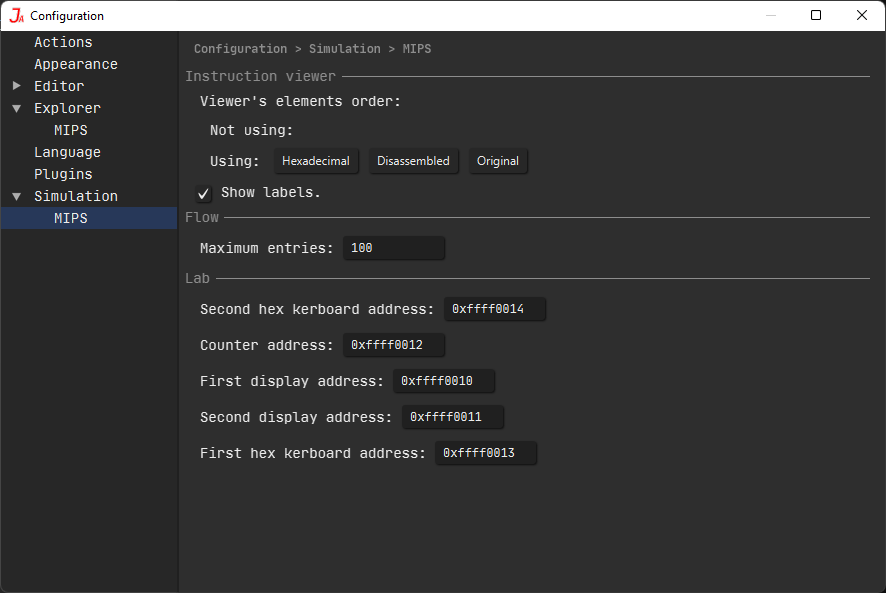
\includegraphics[width=0.8\textwidth]{images/base/jams-config}
    \caption{\textit{Interfaz de configuración}}
    \label{fig:jams-configuracion}
\end{figure}

\subsection{Secciones especiales}\label{subsec:secciones-especiales}

La interfaz de la configuración permite que ciertas gestiones se
gestionen de manera externa por un controlador diferente al de
por defecto.
Estas secciones tienen una estructura totalmente diferente a la
del resto de secciones, lo que permite al usuario modificar
de manera más eficiente sus parámetros.

\section{Acciones}\label{sec:acciones}

Las acciones representan tareas que un usuario puede realizar de manera
\textbf{atómica}.
Las acciones pueden invocarse de diferentes maneras:
desde el menú principal, desde un menú de contexto
o usando una combinación de teclas modificable.
Cabe destacar que las acciones son \textbf{sensibles al contexto}:
una acción solo se podrá ejecutar en un determinado contexto
de la aplicación (el usuario no puede copiar un trozo de texto
en el explorador).

\noindent Los componentes pueden implementar nuevas acciones
creando una nueva clase que extienda $Action$ o $ContextAction$.
La clase $Action$ es la clase básica para las acciones.
Las implementaciones deben implementar el funcionamiento
de la acción en el método $run$.
La clase $ContextAction$ permite que la acción sea
mostrada en un menú contextual.
Las implementaciones de esta clase deben implementar
muchos más métodos que proporcionan información
sobre la viabilidad de la acción en diferentes contextos.

\noindent Los usuarios pueden modificar los atajos de teclado
asociados a una acción en el apartado \textbf{Acciones} de la
configuración.
Una acción puede estar vinculada a más de un atajo de teclado,
lo que le da más libertad de personalización al usuario.
La ventana de acciones contiene una barra de búsqueda que
permite buscar acciones de entre las decenas disponibles.

\begin{figure}[H]
    \centering
    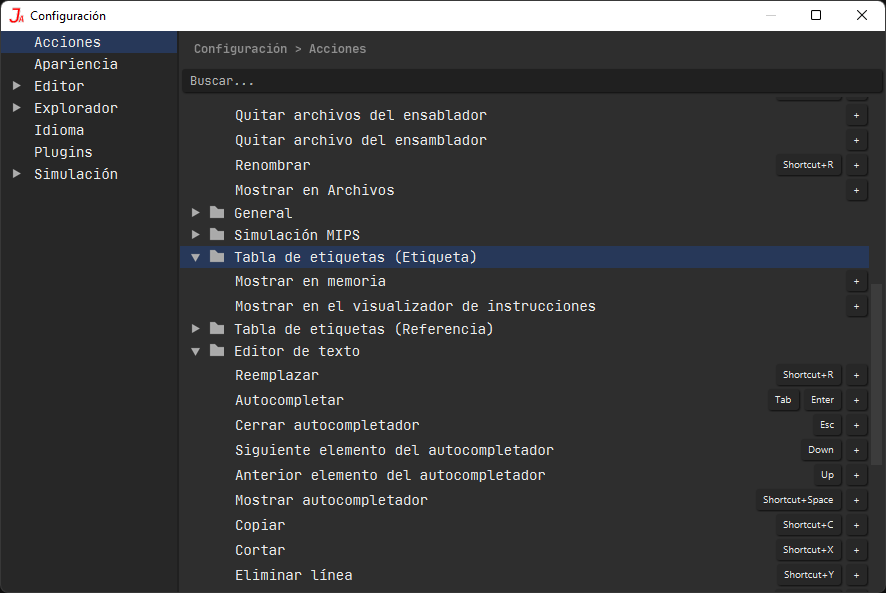
\includegraphics[width=0.8\textwidth]{images/base/jams-config-actions}
    \caption{\textit{Sección de acciones}}
    \label{fig:jams-configuracion-acciones}
\end{figure}

\section{Editor de texto}\label{sec:editor-de-texto}

El editor de texto es la tecnología que más iteraciones
ha sufrido en todo el desarrollo de \textit{JAMS},
siendo uno de los elementos más avanzados de toda
la aplicación.
El editor de texto presenta una arquitectura
\textbf{asíncrona}, y permite gestionar una gran
cantidad de líneas de texto sin bloquear la aplicación.

\subsection{Arquitectura}\label{subsec:arquitectura}

El editor de texto presenta una arquitectura
\textbf{Modelo-Vista-Controlador}:
\begin{itemize}
    \item \textbf{Vista:} la vista está gestionada
    por la librería \textit{RichTextFX}\cite{RICH_TEXT_FX}.
    \textit{RichTextFX} permite añadir estilos
    a secciones del texto.
    La vista está representada por la clase
    $CodeArea$.
    \item \textbf{Controlador:} el controlador está
    gestionado por la clase $CodeFileEditor$.
    Esta clase extiende $CodeArea$, y es la
    encargada de gestionar las entradas del usuario.
    \item \textbf{Modelo:} el modelo está representado
    por la clase $EditorIndex$.
    Las implementaciones de esta clase contienen
    una representación abstracta de los contenidos
    del editor de texto.
    El modelo se actualiza de manera asíncrona.
\end{itemize}

\subsection{Filosofía del modelo}\label{subsec:filosofía-del-modelo}

Debido a la gran complejidad de la arquitectura,
se ha definido una filosofía en el desarrollo
del modelo:
\begin{itemize}
    \item \textbf{Basado en elementos}: cada elemento representa
    un componente en el editor: un comentario, una instrucción,
    una etiqueta, etc.
    Los elementos son \textbf{casi inmutables}:
    solo sus inspecciones, alcances, y posición son mutables.
    \item Los elementos son recreados siempre que una línea
    es editada.
    \item Los elementos almacenan la mínima información
    posible.
    Esta información debe ser buscada usando los métodos
    de consulta proporcionados por el modelo.
    \item Los métodos de consult deben ser lo más rápidos
    posible.
    Las implementaciones por defecto utilizan la
    \textit{Stream API}\cite{STREAM_API} añadida en \textit{Java 8}.
\end{itemize}

\noindent $EditorIndexedElement$ es la la interfaz principal
que representa un elemento.
Esta interfaz define los elementos de posición, tamaño, alcance,
jerarquía y contenido.
Los elementos concretos deben implementar esta interfaz.
Una implementación básica de un elemento puede encontrarse
en la clase $EditorIndexedElementImpl$.

\noindent Si un elemento desea ser referenciado, este debe
implementar la interfaz $EditorReferencedElement$.
Un elemento que implemente esta interfaz será gestionado
de manera diferente por el modelo.
De igual manera, si un elemento desea referenciar
otros elementos, este debe implementar la interfaz
$EditorReferencingElement$.
Estas dos interfaces no son incompatibles:
un elemento puede referenciar y ser referenciado
al mismo tiempo.

\noindent El modelo es un componente \textit{thread-safe}.
Para interactuar con él, un hilo debe reservar el acceso
al modelo y especificar si desea editar su estructura o
solo acceder a sus datos.
Si el hilo modifica el modelo, se crearán dos eventos de tipo
$IndexFinishEditEvent$ y $IndexRequestRefreshEvent$
cuando termine la edición.

\subsection{Actualización del modelo}\label{subsec:actualizacion-del-modelo}

Cuando el controlador sigue el siguiente
protocolo cuando este recibe peticiones de modificación
por parte del usuario:
\begin{itemize}
    \item \textbf{Recolección:} las peticiones cercanas
    en el tiempo son registradas en una lista de peticiones.
    Esta lista es es procesada cuando el usuario deje
    de enviar modificaciones.
    \item \textbf{Compresión:} se descartan las peticiones
    de modificación que no van a tener efecto en el modelo.
    El caso más común de modificaciones sin efecto sería
    el de una cadena de modificaciones en una misma línea:
    solo el estado de la línea en la modificación final
    tendrá efecto en el modelo.
    \item \textbf{Actualización:} se genera una tarea
    asíncrona que modifica el modelo en base a las
    peticiones.
    \item \textbf{Finalización:} una vez el modelo
    es modificado, se envían una serie de eventos
    a la vista para que esta actualice el estilo
    de las líneas visibles.
\end{itemize}

\subsection{Estructura del modelo}\label{subsec:estructura-del-modelo}

El modelo presenta una arquitectura jerárquica de elementos:
un elemento tiene un padre y puede tener varios hijos.
Cada elemento contiene su posición inicial en el archivo, la
longitud de su representación y la representación en sí.
Esta estructura puede considerarse una implementación de un
\textit{Rope}\cite{ROPES}, una estructura de dastos muy
utilizada para editores de texto.

\begin{center}
    \basictree{
        [Instruction 0 13 sw \$s0 0(\$s2)
        [Mnemonic 0 2 sw]
        [Parameter 3 3 \$s0
        [Register 3 3 \$s0]
        ]
        [Parameter 7 6 0(\$s2)
        [Immediate 7 1 0]
        [Register 9 3 \$s2]
        ]
        ]
    }
\end{center}

\noindent Los nodos hoja pueden implementar la interfaz
$EditorIndexStyleableElement$, permitiendo inyectar
estilos en la vista del editor de texto.
Esta interfaz solo presenta un método que pide una lista
de estilos.
\textit{JAMS} es el encargado de inyectar dichos estilos
en el editor cuando sea necesario.

\begin{figure}[H]
    \centering
    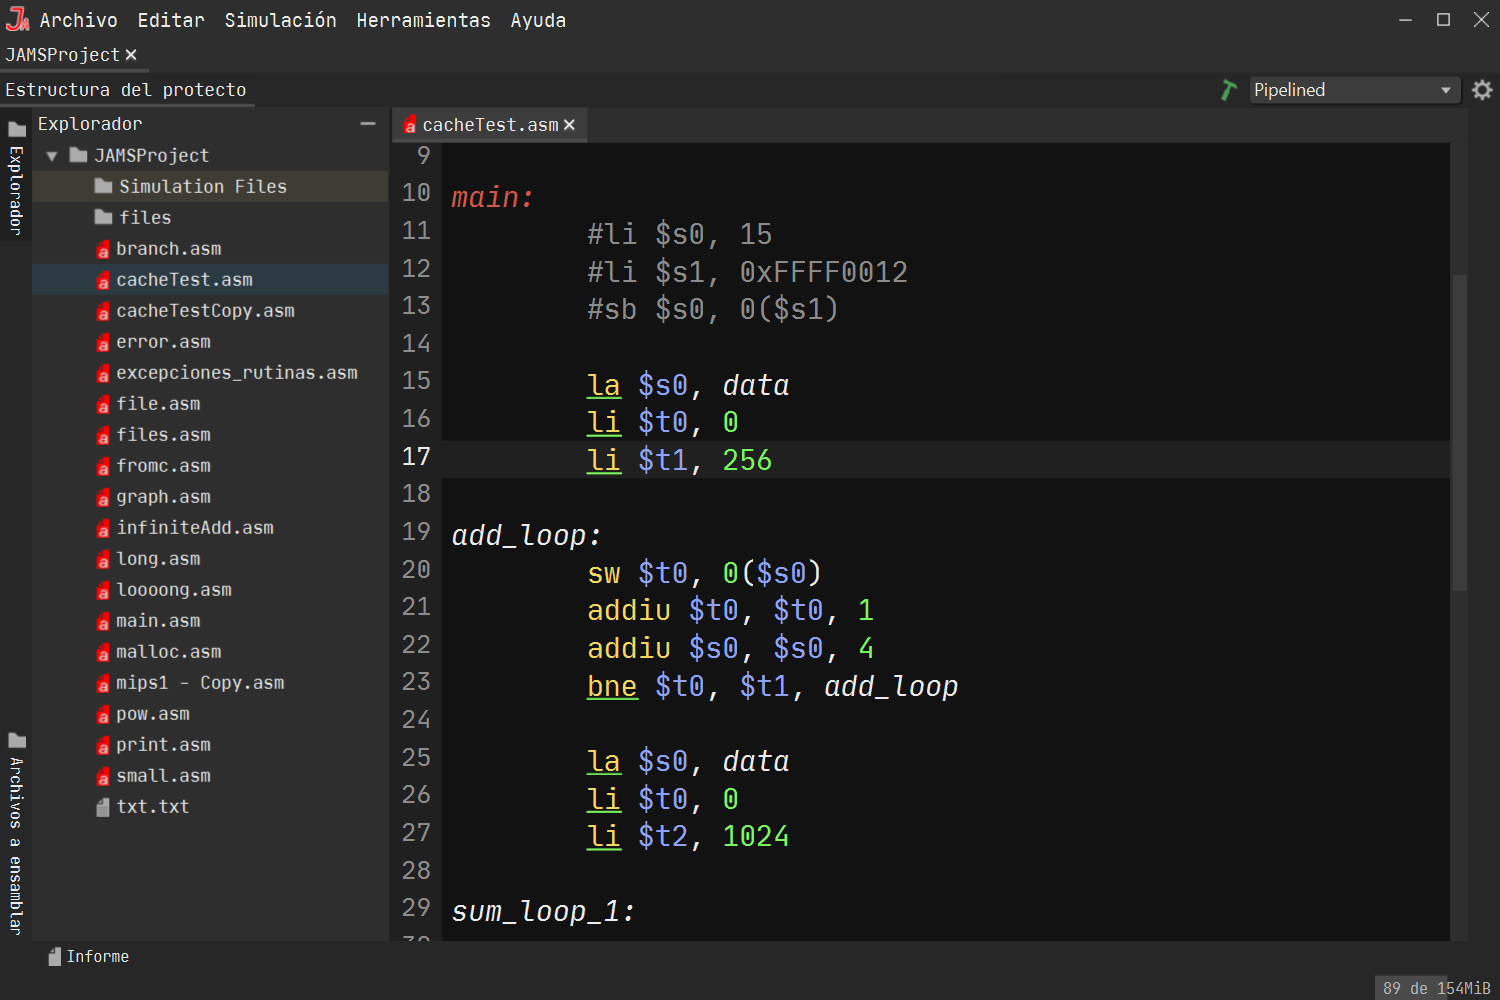
\includegraphics[width=0.8\textwidth]{images/base/jams-text-editor}
    \caption{Editor de texto con estilos inyectados}
    \label{fig:jams-editor-texto}
\end{figure}

\subsection{Referencias entre modelos}\label{subsec:referencias-entre-modelos}

Un modelo puede tener \textbf{referencias a elementos
presentes en otros modelos}.
Este es el caso de las etiquetas y macros globales.
La clase $ProjectGlobalIndex$ permite la
comunicación entre modelos, actuando de intermediador.
Solo los elementos que están dentro de los archivos
de la lista de archivos a ensamblar serán tomados en cuenta.
Para evitar interbloqueos, todas las modificaciones
realizadas en un proyecto son gestionadas en el
mismo hilo.

\subsection{Implementaciones}\label{subsec:implementaciones}

\textit{JAMS} incorpora implementaciones básicas de los
diferentes componentes usados en el editor.
Una de las implementaciones más importantes es la que está
definida en la clase $EditorLineIndex$, la cual
implementa un modelo donde cada línea representa una
unidad autocontenida.

\noindent Otras implementaciones serían la de elementos
básicos y comunes en diferentes lenguajes ensamblador:
las etiquetas, las macros, las llamadas a macros o
los comentarios son ejemplos de elementos ya definidos.

\subsection{Autocompletación}\label{subsec:autocompletacion}

\textit{JAMS} aprovecha los datos proporcionados por
el modelo para implementar una interfaz de autocompletación
que el usuario puede usar en el editor.

\begin{figure}[H]
    \centering
    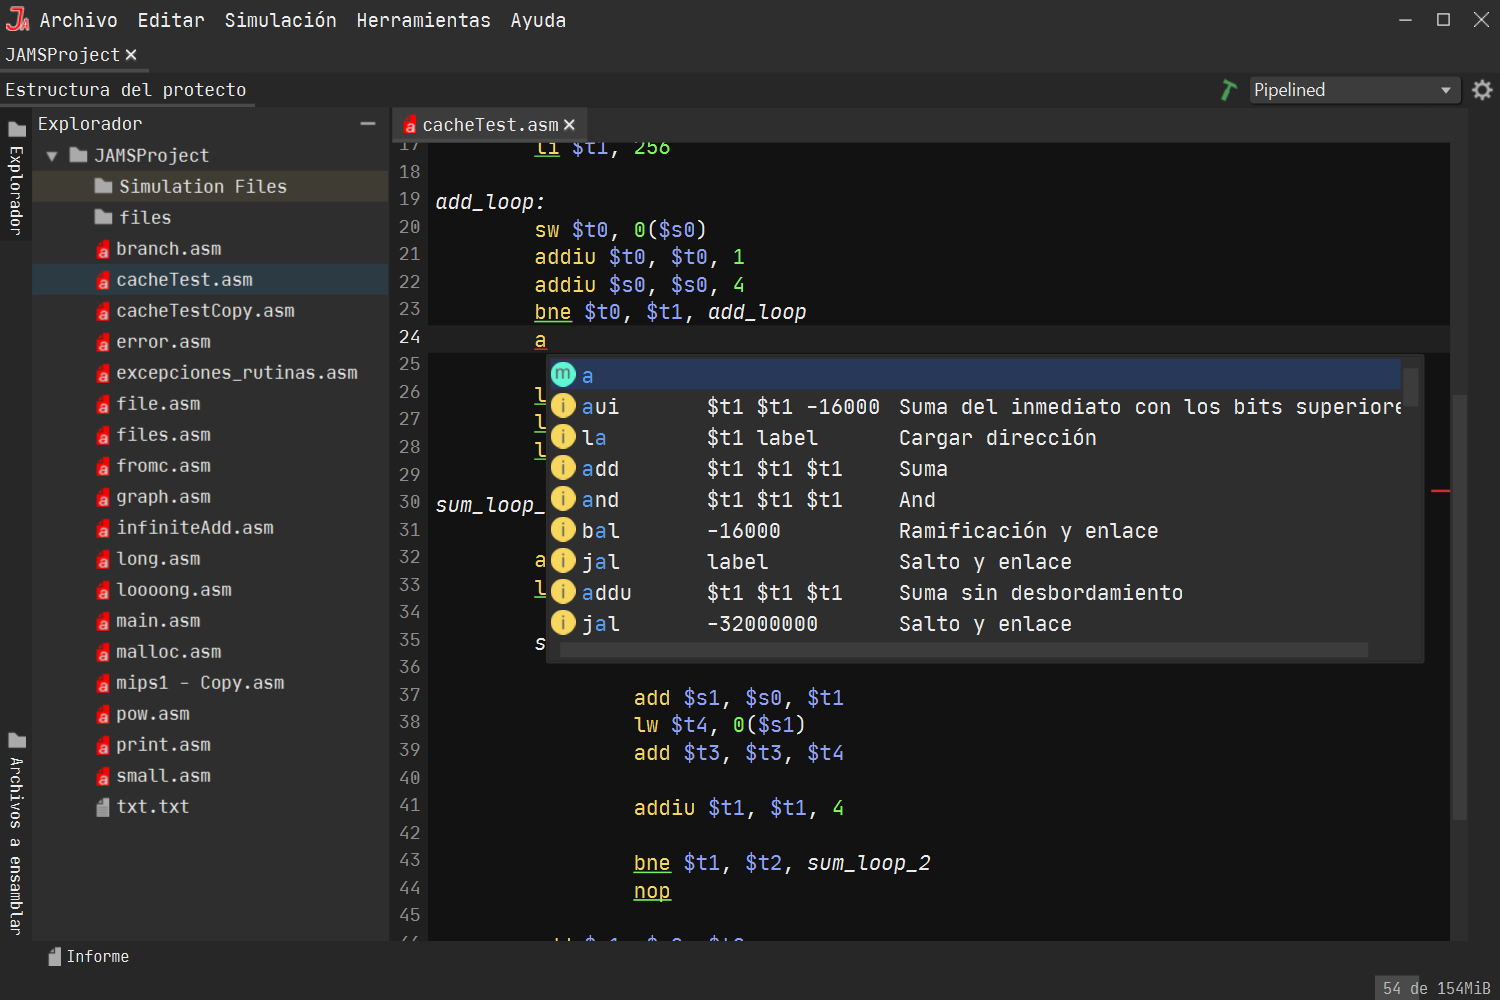
\includegraphics[width=0.8\textwidth]{images/base/jams-autocompletion}
    \caption{Autocompletador del editor de texto}
    \label{fig:jams-autocompletador}
\end{figure}

\noindent Igual que el propio editor de texto, esta interfaz
presenta una estructura modelo-vista-controlador:

\begin{itemize}
    \item \textbf{Controlador:} implementado en dos partes.
    \textit{JAMS} implementa las acciones de la interfaz,
    mientras que el desarrollador debe implementar el
    generador del modelo.
    \item \textbf{Modelo:} contiene los candidatos de
    la interfaz.
    \item \textbf{Vista:} implementa la interfaz que
    muestra los candidatos del modelo.
    \textit{JAMS} implementa una vista por defecto,
    pero los desarrolladores pueden implementar una
    vista propia.
\end{itemize}

\subsection{Documentación}\label{subsec:documentacion}

Como característica final, el editor de texto presenta
una interfaz de documentación que los proyectos
pueden utilizar para documentar sus diferentes
elementos.
Se puede acceder a la documentación con la secuencia por defecto
\textbf{Ctrl + Q}.

\begin{figure}[H]
    \centering
    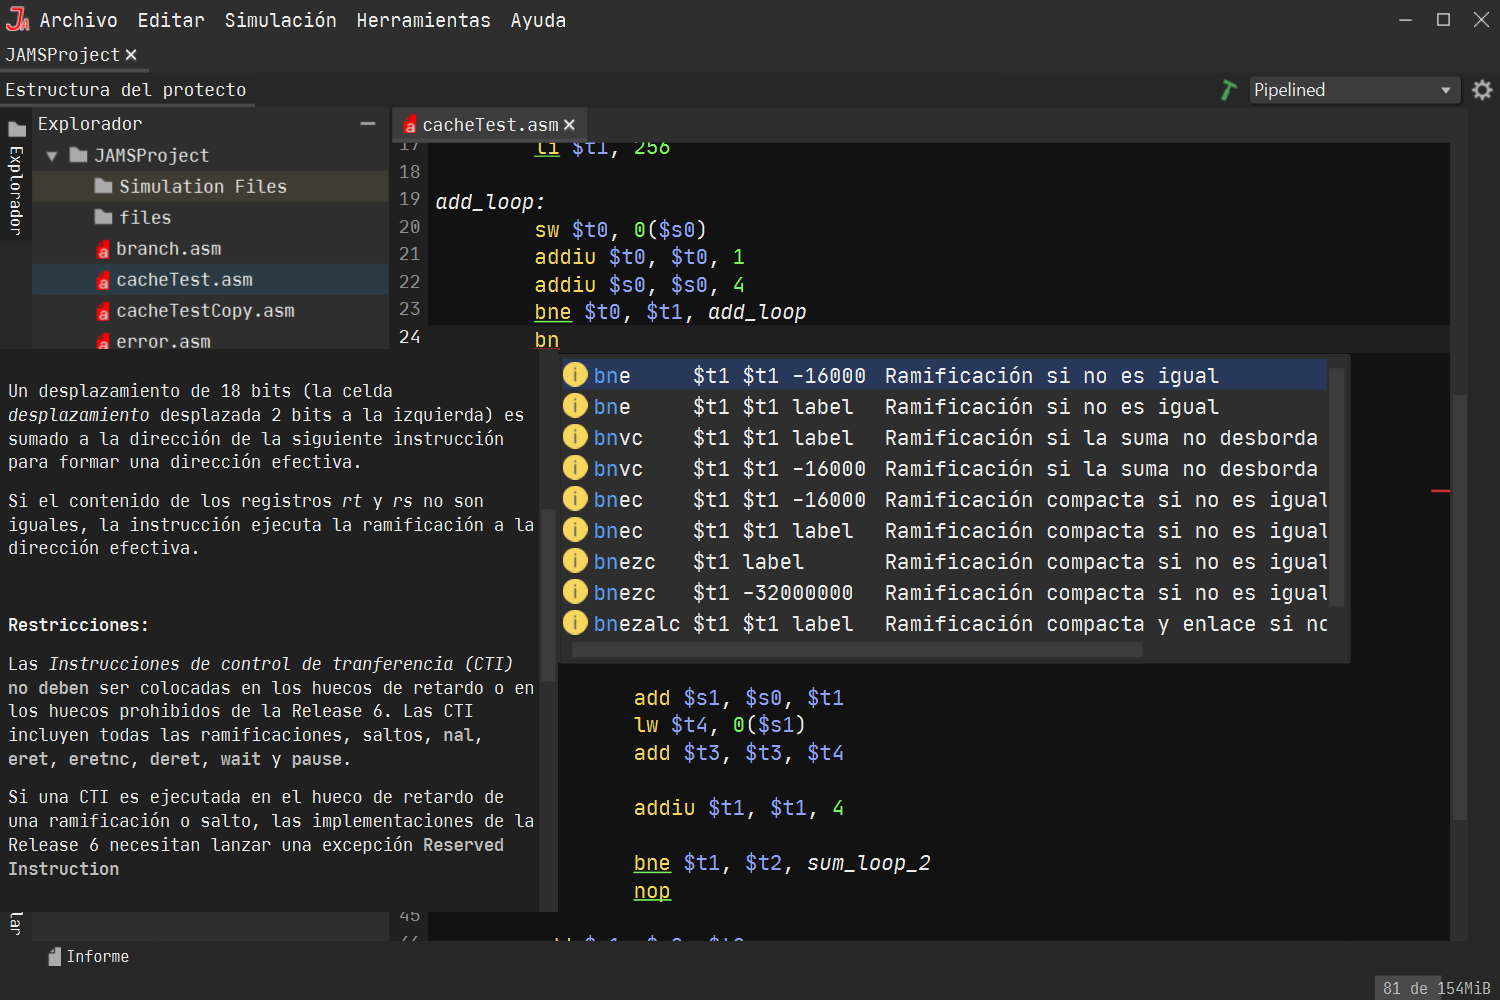
\includegraphics[width=0.8\textwidth]{images/base/jams-documentation}
    \caption{Documentación en el editor de texto}
    \label{fig:jams-documentacion}
\end{figure}
    \chapter{Entorno de desarrollo \textit{MIPS32}}\label{ch:entorno-de-desarrollo-mips32}

El desarrollo de \textit{JAMS} está dividido en dos secciones:
la aplicación base y el entorno de desarrollo \textit{MIPS32}.
\textit{JAMS} da soporte al lenguaje ensamblador \textit{MIPS32}
creando una \textbf{capa sobre la aplicación base},
aprovechando todas las herramientas y características explicadas anteriormente.
En este capítulo se abordarán las capacidades de este entorno,
documentando el ensamblador, el simulador y el editor junto
con sus componentes esenciales.


\section{Editor de código \textit{MIPS32}}\label{sec:editor-de-codigo-mips32}

\textit{JAMS} aprovecha la tecnología creada en el entorno base
para el editor de código \textit{MIPS32}.
Este editor se complementa con diferentes nodos presentes en la
aplicación.

Cuando el usuario abre un proyecto y desea editar su código,
debe seleccionar el archivo que desea modificar.
Esto se consigue gracias a la herramienta \textbf{explorador}\ref{fig:jams-explorer-text-hover}, la cual
muestra una representación en forma de árbol de la estructura del proyecto.
El usuario puede expandir y contraer carpetas, así como crear, borrar y
mover archivos.
Si el usuario usa el doble clic sobre un archivo editable, este se abrirá
en el editor.

\begin{figure}[h]
    \centering
    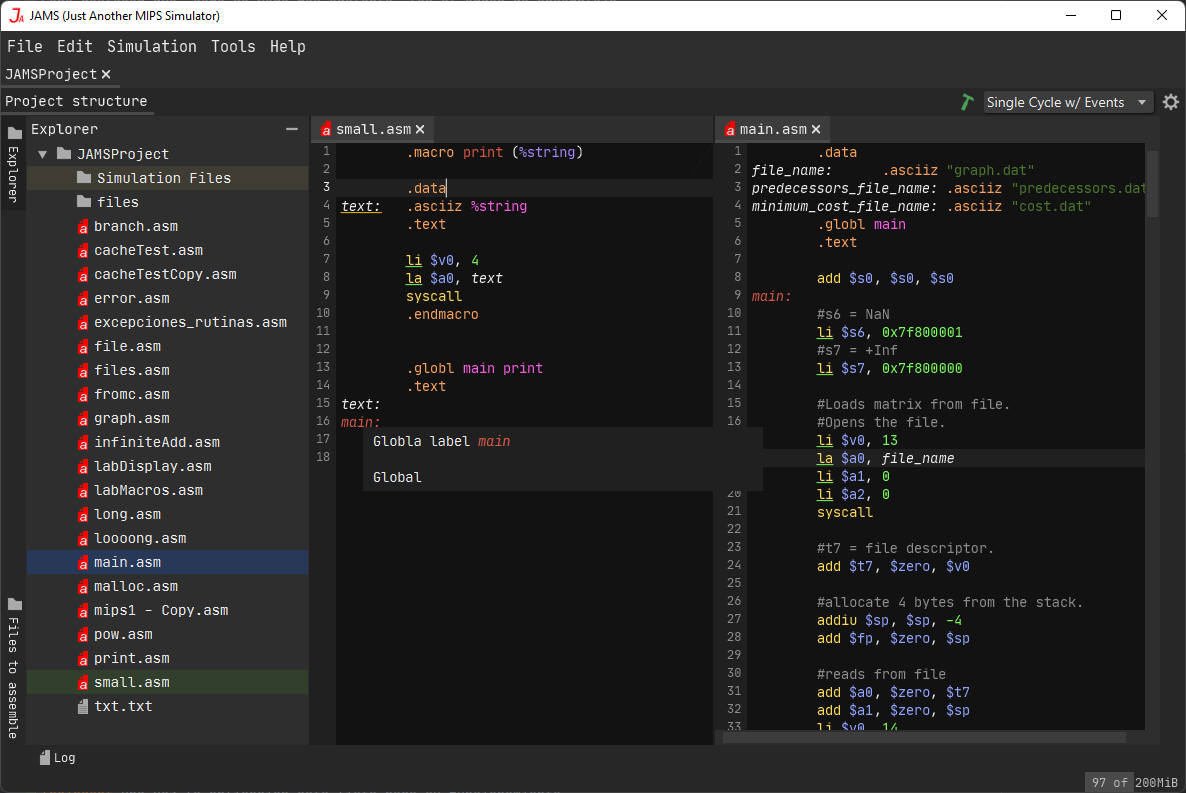
\includegraphics[width=0.8\textwidth]{images/mips/jams-text-hover}
    \caption{Explorador e información sobre un elemento del editor}
    \label{fig:jams-explorer-text-hover}
\end{figure}


El explorador presenta un menú contextual donde el usuario
puede ejecutar varias acciones sobre las carpetas y los archivos
del proyecto.
Una de las opciones más particulares es la opción de añadir o eliminar
archivos de código a la lista de archivos fuente para ensamblar.
Al ser \textit{JAMS} un entorno de desarrollo basado en \textbf{proyectos},
se ha de proporcionar una manera de incluir o excluir archivos de
la aplicación resultante.
Con este sistema tan sencillo, el usuario podrá elegir qué archivos se deben ensamblar.
Los archivos que se ensamblarán estarán marcados en \textbf{verde} en el explorador,
y aparecerán en orden en el nodo \textbf{archivos para ensamblar}.
Como se verá más adelante, cabe destacar que el orden de ensamblaje
es importante, por lo que esta herramienta permite ordenar de una manera
sencilla dichos archivos.

Una vez el usuario haya abierto el archivo para editar, todo su código
aparecerá en la herramienta principal de la sección: \textbf{el visualizador
de archivos}.
Esta herramienta permite mostrar diferentes editores dependiendo del tipo
de archivo abierto.
En la versión sin componentes de \textbf{JAMS}, el editor permite visualizar
imágenes y editar archivos de texto.
En el caso de estos últimos, solo los archivos escritos en
lenguaje ensamblador presentan ayudas, como pueden ser el autocompletador,
el resaltador o la documentación.

El visualizador de archivos puede tener varios archivos abiertos
al mismo tiempo.
Cada archivo estará representado por una pestaña que podrá cerrarse.
El usuario podrá arrastrar una de las pestañas a un lado del visualizador
para mostrar dos o más editores al mismo tiempo.

El editor de código \textit{MIPS32} puede considerarse un editor
de texto \textbf{inteligente}: gracias a las librerías creadas en la sección
anterior, es capaz de convertir el texto puro en los diferentes componentes
ensamblador que representa.
El editor también tiene conocimiento de las referencias y el alcance de
todas las etiquetas y macros, tanto en el propio archivo que se stá editando
como en el resto de archivos que se van a ensamblar.
Toda esta información puede ser visualizada por el usuario manteniendo
durante un segundo el ratón encima de un elemento, como se observa
en la figura \ref{fig:jams-explorer-text-hover}.

Antes de ensamblar el proyecto el usuario deberá \textbf{crear una configuración}
con todos los parámetros del ensamblador y del simulador deseados.
Esto se consigue pulsando el botón \textbf{configuración} en la parte
superior derecha de la aplicación.
En este menú, el usuario podrá seleccionar el tipo de arquitectura,
el tipo de memoria, las llamadas a sistema que se desean usar,
\newODR{o} el número y tipos de caché que se desean utilizar, entre otras
muchas opciones, como se puede observar en la figura \ref{fig:jams-configuration}.

\begin{figure}[h]
    \centering
    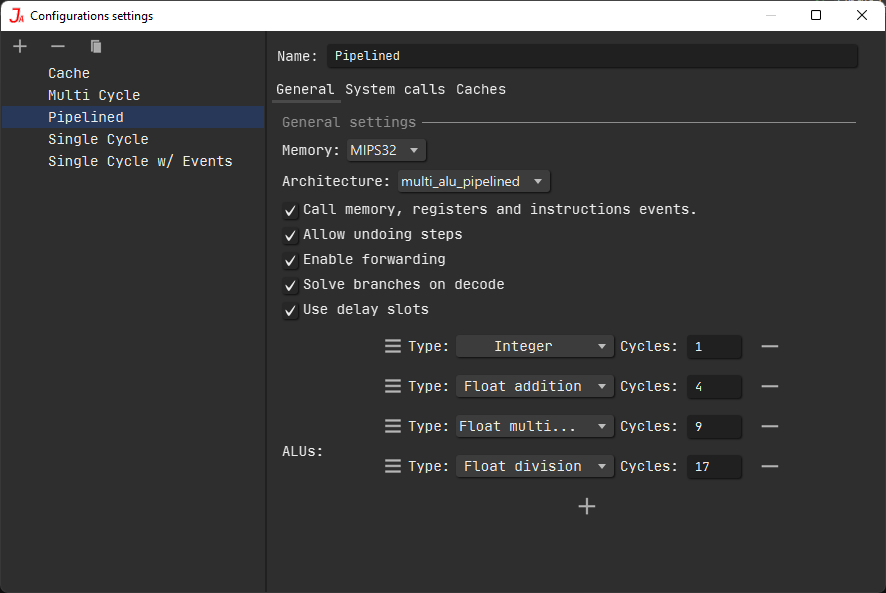
\includegraphics[width=0.8\textwidth]{images/mips/mips-configuration}
    \caption{Configuración de la ejecución de un proyecto}
    \label{fig:jams-configuration}
\end{figure}

Esta configuración se utilizará únicamente en el proyecto
donde se ha creado, y el usuario podrá crear por cada proyecto
un número indeterminado de configuraciones.
De esta manera, el usuario podrá probar su proyecto en una infinidad
de configuraciones diferentes sin tener que generar un proyecto
diferente por cada configuración.
El usuario podrá seleccionar la configuración que desea ejecutar en
el menú desplegable situado inmediatamente a la izquierda del
botón de configuración.

Finalmente, el usuario podrá llamar al ensamblador pulsando el botón
\textbf{construir proyecto}, representado por un martillo verde.
Una vez pulsado, se desplegará un informe que mostrará el resultado del ensamblaje.
Si el resultado es positivo y el código se ha ensamblado,
aparecerá en el proyecto una nueva ventana de simulación,
permitiendo al usuario simular el código que acaba de ensamblar.
Si el resultado no es positivo, el informe mostrará el error producido
por el ensamblador.
Cabe destacar que un usuario puede tener diferentes simulaciones abiertas
al mismo tiempo, lo cual amplía las posibilidades de uso de la
aplicación.


\section{Ensamblador \textit{MIPS32}}\label{sec:ensamblador-mips32}

El ensamblador \textit{MIP32} de \textit{JAMS} es un ensamblador avanzado
útil para ensamblar proyectos \textit{MIPS32}.
Este ensamblador soporta características avanzadas empleadas
comúnmente al programar en ensamblador, como las macros,
las etiquetas globales o las referencias relativas.
El ensamblador ensambla el código de un proyecto en \textbf{cuatro pasos}:
descubrimiento, expansión, asignación de direcciones y asignación de valores.
Se utilizará el siguiente programa para comentar los diferentes pasos del ensamblador:

\begin{lstlisting}[frame=single,label={lst:example.asm}]
    .macro print ( %string )
    .data
text:   .asciiz %string
    .text
    la $a0, text
    li $v0, 4
    syscall
    .endmacro

    .macro printJams ()
    print ("Welcome to JAMS!\n")
    .endmacro

    .text
    .globl main print
main:
local:
    printJams ()
\end{lstlisting}

\subsection{Descubrimiento}\label{subsec:descubrimiento}

En este paso el texto del proyecto se \textbf{descompone en sus primitivas},
permitiendo al ensamblador entender los diferentes componentes de cada línea.
Al final de este paso, las etiquetas globales y las etiquetas del archivo
(etiquetas no definidas dentro de una macro) \textbf{son registradas sin
ningún valor asignado}.
Las macros de cada archivo también son registradas.
El identificador de una macro se define por su nombre concatena\newODR{n}do
un carácter $-$ al número de parámetros que necesitan.
Este procedimiento se realiza para dar soporte a la sobrecarga de macros.
En el caso de la macro $print$, su identificador sería $print-1$.

\begin{lstlisting}[frame=single,label={lst:descubrimiento}]
Etiquetas globales:
main - XXXXXXXX

Etiquetas del archivo:
local - XXXXXXXX

Macros globales:
print-1

Macros del archivo:
printJams-0
\end{lstlisting}

\subsection{Expansión}\label{subsec:expansion}

En este paso, se invocan las llamadas a las macros,
insertando el código de cada macro en la posición de la llamada,
expandiéndola y llevando a cabo el primer paso del ensamblaje.

\begin{lstlisting}[frame=single,label={lst:expansion}]
main:
local:
    # Macro printJams-0
    # Macro print-1
    .data # Data returns the previous address.
text:   .asciiz "Welcome to JAMS!\n"
    .text
    la $s0, text
    li $v0, 4
    syscall
    # Endmacro print-1
    # Endmacro printJams-0
\end{lstlisting}

\subsubsection{Alcance}\label{subsubsec:alcance}

Las etiquetas y macros que están dentro de una macro
\textbf{tienen un alcance diferente al del archivo}.
Si la macro es global, el alcance es considerado hijo del alcance global
y no podrá acceder a las etiquetas del archivo que lo invoca.
Si la macro es local, el alcance es considerado hijo del alcance del archivo.

Cuando un alcance es hijo de otro alcance,
\textbf{el hijo podrá acceder a las etiquetas y macros de su padre}.
El hijo también podrá definir nuevas etiquetas y macros con el mismo
identificador que una etiqueta o macro de su padre.
Aunque este comportamiento está permitido, \textbf{el hijo solo podrá acceder
al elemento que él define}.
Esta funcionalidad es llamada \textbf{ocultamiento o \textit{shadowing}}.

\subsection{Asignación de direcciones}\label{subsec:asignacion-de-direcciones}

Una vez el ensamblador haya expandido las macros,
se asignan las direcciones de todas las instrucciones,
etiquetas y directivas que requieran una dirección.
Estas direcciones se asignan de manera secuencial.
Existen directivas que pueden modificar el flujo de la asignación,
como es el caso de la directiva $.text$.

\begin{lstlisting}[frame=single,label={lst:address-assignation}]
main:
local:
                    # Macro printJams-0
                    # Macro print-1

0x00400000          .data # Data returns the previous address.
0x10010000      text:    .asciiz "Welcome to JAMS!\n"
0x10010010          .text

                    # la is a pseudo-instruction and
                    # it will be split in two instructions
0x00400000          la $s0, text
0x00400008          li $v0, 4
0x0040000c          syscall

                    # Endmacro print-1
                    # Endmacro printJams-0
\end{lstlisting}

\subsection{Asignación de valores}\label{subsec:asignacion-de-valores}

Como paso final, el ensamblador insertará en memoria los valores
que representan las directivas e instrucciones.

\begin{lstlisting}[frame=single,label={lst:value-assignation}]
                    # Macro printJams-0
                    # Macro print-1

0x10010000          Welcome to JAMS!\n\0
0x00400000          0x3c011001 # la $a0, text
0x00400004          0x34240000
0x00400008          0x24020004 # li $v0, 4
0x0040000c          0x0000000c # syscall

                    # Endmacro print-1
                    # Endmacro printJams-0
\end{lstlisting}

\subsection{Características avanzadas}\label{subsec:características-avanzadas}

El ensamblador permite el uso de técnicas avanzadas en
el desarrollo de aplicaciones en lenguaje ensamblador.

\subsubsection{Referencias relativas}\label{subsubsec:referencias-relativas}

Una directiva o instrucción puede \textbf{referenciar a una etiqueta de manera
relativa} con las referencias especiales $+$ y $-$.
La referencia $+$ hace referencia a la etiqueta siguiente.
La referencia $-$ hace referencia a la etiqueta anterior.
Las referencias relativas \textbf{solo pueden hacer referencia
a etiquetas del mismo alcance}.
No pueden hacer referencia a etiquetas de un alcance mayor.

\begin{lstlisting}[frame=single,label={lst:relative-reference}]
main:
    li $s0, 0
    li $s1, 10
loop:
    printJams ()
    addi $s0, $s0, 1
    bne $s0, $s1, -
\end{lstlisting}

\subsubsection{Macros anidadas}\label{subsubsec:macros-anidadas}

Una macro puede ser definida dentro de otra macro,
lo que se conoce como \textbf{macro anidada}.
Esta macro solo podrá ser accedida en el alcance de la macro
en la que está declarada.

\begin{lstlisting}[frame=single,label={lst:nested-macro}]
    .macro printJams ()
    .macro print (%string)
    .data
text:   .asciiz %string
    .text
    la $a0, text
    li $v0, 4
    syscall

    .endmacro
    print ("Welcome to JAMS!\n")
    .endmacro
\end{lstlisting}

\subsection{Detalles finales}\label{subsec:detalles-finales}

Como detalle final, cabe destacar que este ensamblador es totalmente personalizable.
Los componentes pueden añadir, eliminar y modificar las instrucciones y directivas
utilizadas.
La adición de directivas por parte de los componentes permite
\textbf{modificar el comportamiento} del ensamblador, añadiéndole
nuevas funcionalidades.

Añadir una instrucción o una directiva es muy sencillo en \textit{JAMS}:
un componente únicamente debe añadir una nueva instrucción o
una nueva directiva (representadas por clases) a un conjunto de
instrucciones o directivas ya existente, o crear ese conjunto y registrarlo
con la \textit{API} de \textit{JAMS}.
A este nuevo elemento se le puede añadir un nombre traducible y documentación
a través de un paquete de idiomas.

\section{Simulador}\label{sec:simulador}

Un simulador es una pieza de \textit{software} que imita el comportamiento
de un dispositivo.
\textit{JAMS} implementa diversos simuladores para las diferentes
arquitecturas \textit{MIPS32}.
En \textit{JAMS} toma mucho más peso el enfoque de la
\textbf{simulación} a nivel de circuito, permitiendo al usuario
conocer el funcionamiento de su aplicación en la arquitectura que desee.
Esto no significa que \textit{JAMS} no optimice la ejecución de código:
todos los componentes están altamente optimizados, pudiendo
realizar simulaciones a una velocidad de 40 MHz.

\subsection{Arquitecturas disponibles}\label{subsec:arquitecturas-disponibles}

Actualmente, \textit{JAMS} permite ejecutar el código
en tres arquitecturas \textit{MIPS32} diferentes:
\begin{itemize}
    \item \textbf{Uniciclo}: es la arquitectura más sencilla y
    mejor optimizada.
    Se ha creado con la velocidad en mente, optando por una
    política de \textbf{cero liberación de memoria}: se crean los mínimos
    objetos posibles, y estos no se liberarán de la memoria hasta que
    la simulación haya terminado.
    Esta política evita que el recolector de basura interfiera en la
    ejecución del simulador, aunmentando su velocidad de ejecución.
    \item \textbf{Multiciclo:} simula una arquitectura
    \textit{MIPS32} multiciclo.
    Es mucho más lenta que la arquitectura uniciclo, ya que requiere
    tener muchos más conceptos en cuenta.
    Las implementaciones de las ejecuciones en esta arquitectura
    se han diseñado para ser aprovechadas en arquitecturas más
    complejas, definiendo las lecturas y escrituras de sus
    registros y compartiendo una interfaz transparente para los saltos.
    \item \textbf{Segmentada con varias \textit{ALUs}}: simula
    una arquitectura segmentada o \textit{pipelined} donde coexisten varias
    unidades aritmético-lógicas.
    Esta arquitectura aprovecha mucho código de la arquitectura
    multiciclo, y tiende a ser mucho más lenta.
    Los usuarios pueden modificar el número y tipo de las unidades
    aritmético-lógicas, así como el número de ciclos que requiere
    cada una para completar una operación.
\end{itemize}

\subsection{Estructura del simulador}\label{subsec:estructura-del-simulador}

Independientemente de la arquitectura, todas las simulaciones presentan
la misma estructura básica, idéntica en su base al editor.
Al ejecutar una simulación, el usuario encuentra como nodo principal
un \textbf{visualizador de instrucciones}, mostrado en la figura \ref{fig:jams-simulation}.
Esta herramienta permite visualizar todas las instrucciones ensambladas
junto a su dirección de memoria, su valor en hexadecimal y
su origen.
El orden de estos valores se puede cambiar en la configuración.
El visualizador también informa sobre las \textbf{instrucciones que se van
a ejecutar} en el siguiente ciclo y, si la arquitectura tiene varias
etapas, mostrará qué etapa ejecutará.
Si la aplicación simulada tiene código para el modo \textit{kernel},
este se mostrará en una pestaña aparte.

\begin{figure}[h]
    \centering
    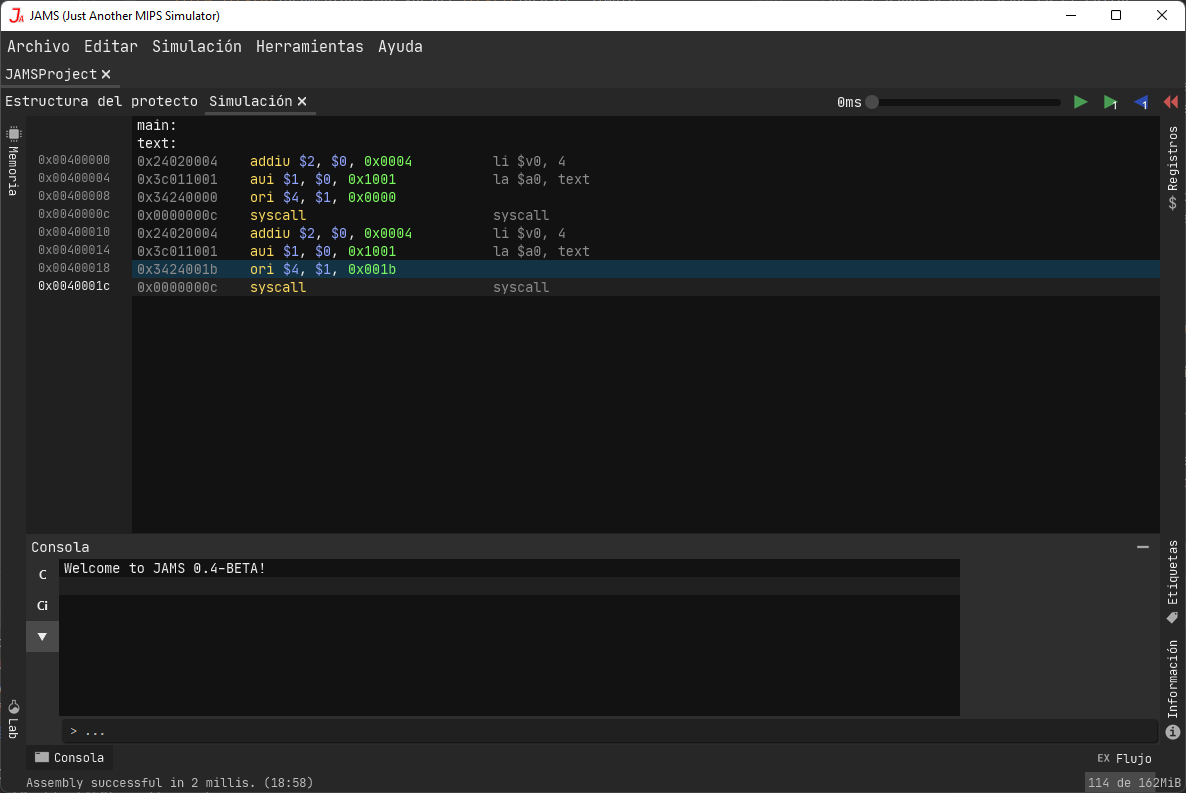
\includegraphics[width=0.8\textwidth]{images/mips/jams-simulation}
    \caption{Interfaz de usuario del simulador}
    \label{fig:jams-simulation}
\end{figure}

Los \textbf{botones de control} del simulador se encuentran
en la parte superior derecha.
Estos botones permiten empezar o parar la simulación, ejecutar un
único ciclo, deshacer un ciclo o reiniciar por completo la simulación.
Esta sección también contiene una barra deslizable que permite controlar
la velocidad a la que se ejecuta la simulación.

La ejecución del simulador es totalmente asíncrona, lo cual
impide bloqueos de interfaz cuando una aplicación se está ejecutando.
Todos los componentes y herramientas que accedan al simulador
deberán sincronizarse con el hilo del simulador.

El simulador tiene integradas \textbf{diversas herramientas} que complementan
al visualizador de instrucciones, permitiendo visualizar y modificar varios
aspectos de la ejecución de un programa.

El nodo más importante es la herramienta de \textbf{memoria},
la cual permite al usuario visualizar y editar el estado de la memoria
en el instante actual.
El usuario puede seleccionar el \textbf{modo de representación} de los valores
de la memoria de entre una gran variedad, pudiendo elegir formatos
frecuentemente utilizados como por ejemplo el formato hexadecimal,
o formatos específicos como el \textit{RGB}.
Por último, esta herramienta también permite visualizar el \textbf{estado
de las cachés} del simulador.
Esta información se complementa mediante la herramienta \textbf{cachés},
la cual informa sobre los fallos y aciertos de las cachés,
además de presentar un informe completo sobre sus acciones.

\begin{figure}[h]
    \centering
    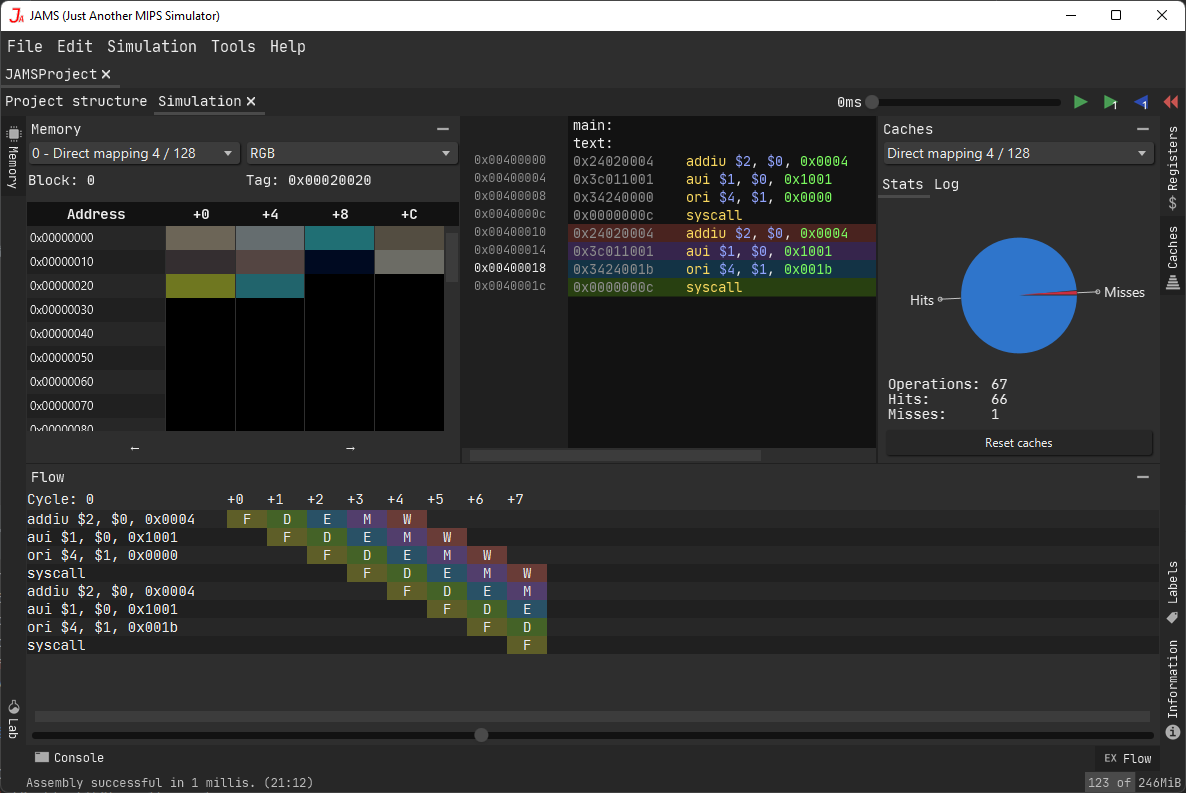
\includegraphics[width=0.8\textwidth]{images/tools/jams-memory-cache-flow}
    \caption{Las herramientas memoria, cachés y flujo en funcionamiento}
    \label{fig:jams-memory-cache-flow}
\end{figure}

Otro nodo muy relevante es la herramienta \textbf{flujo},
que registra el estado de todas las instrucciones en cada ciclo
de ejecución.
De esta manera, el usuario podrá saber de un vistazo qué flujo
ha seguido su aplicación en la arquitectura seleccionada.

Como último nodo crucial se encuentra la herramienta
\textbf{laboratorio}, que permite al usuario simular
dos visualizadores de siete segmentos, un teclado hexadecimal
y un contador, además de poder generar interrupciones \textit{hardware}
y \textit{software}.

El simulador cuenta con muchos nodos más, como son la
herramienta \textbf{registros}, que permite visualizar y modificar
todos los registros del simulador, la herramienta \textbf{etiquetas},
que guarda las referencias de las etiquetas usadas por el usuario
en el editor, la herramienta \textbf{información}, que muestra
información muy básica y general de la simulación y la
herramienta \textbf{consola}, que permite recibir y enviar
mensajes a la aplicación.

\subsection{Aspectos técnicos}\label{subsec:aspectos-tecnicos}

En esta sección se detallarán brevemente los aspectos técnicos
más relevanes del simulador.

\subsubsection{Memoria}\label{subsubsec:memoria}

La memoria es la parte del simulador donde se guardan los datos
y las instrucciones de una aplicación.
La memoria de la arquitectura \textit{MIPS32} es una memoria de 4 GB
($2^{32}$ bytes) separada en las siguientes secciones:

\begin{figure}[H]
    \centering
    \resizebox{\textwidth}{!}{%
        \begin{tabular}{|l|l|l|l|}
            \hline
            Sección       & Tipo         & Primera dirección & Uso                                                              \\ \hline
            Reserved      & Kernel Level & 0xFFFF0000        & Sección usada para leer y escribir de componentes.               \\ \hline
            Kernel Data   & Kernel Level & 0x90000000        & Datos estáticos del \textit{kernel}.                             \\ \hline
            Kernel text   & Kernel Level & 0x80000000        & Instrucciones del \textit{kernel}.                               \\ \hline
            Stack Segment & User Level   & ↓                 & Pila.                                                            \\ \hline
            Dynamic Data  & User Level   & ↓                 & Memoria reservada en tiempo de ejecución.                        \\ \hline
            Static Data   & User Level   & 0x10000000        & Datos estáticos generados por las directivas al ensamblar.       \\ \hline
            Text Segment  & User Level   & 0x04000000        & Instrucciones del programa.                                      \\ \hline
            Reserved      & Kernel Level & 0x00000000        & Sección usada por el sistema operativo. Sin uso en el simulador. \\ \hline
        \end{tabular}%
    }
    \caption{Estructura de la memoria en \textit{MIPS32}}
    \label{fig:memory-table}
\end{figure}

Reservar 4 GB de memoria para cada simulación no es una buena idea:
ocuparía una gran parte de la RAM de un computador y
la mayor parte de ese espacio no se utilizaría.
Para evitar este problema existen varias técnicas para la
implementación de la memoria:
\begin{itemize}
    \item Limitar la memoria de cada sección.
    Esta técnica es la empleada en el simulador \textit{MARS}.
    \item Partir las secciones en sub-secciones.
\end{itemize}

\textit{JAMS} implementa la segunda opción:
cada sección de memoria se separa en bloques de 4 KB\@.
Estas secciones no se reservan en memoria
hasta que son necesarias.
Con esta implementación, se reserva un array inicial de
$2^{22}$ ($2^{32}$ / $2^{12}$) entradas, lo que equivaldría
a 8 MB\@.
Según el uso de la memoria dentro del simulador,
se irán reservando fragmentos adicionales de 4 KB\@.

\subsubsection{Cachés}\label{subsubsec:caches}

Las cachés son memorias pequeñas y rápidas situadas entre
la memoria y el procesador.
Los computadores actuales suelen tener varios niveles de caché.
En \textit{JAMS}, las memorias funcionan de manera muy similar.
Tanto las cachés como las memorias implementan la interfaz $Memory$.
Esta interfaz define los métodos de lectura y escritura.
Cuando un simulador necesita leer o escribir en la memoria,
llama al método correspondiente en su memoria.
Lo que no sabe el simulador es que su \textbf{memoria puede ser una caché}
con una referencia a otra memoria.
Cuando una se invoca a una caché en una operación de lectura o escritura,
es ella quien gestiona la operación y,
si es necesario, accede a la memoria de nivel inferior que tiene como referencia.
Con esta sencilla arquitectura se genera una jerarquía de memorias
muy similar a la que encontramos en computadores reales.

Actualmente, \textit{JAMS} soporta tres tipos básicos
de cachés: \textbf{cachés por correspondencia directa},
\textbf{cachés asociativas} y \textbf{cachés asociativas por conjuntos}.
Todos los tipos de cachés soportan tanto el modo \textit{write-back}
como el modo \textit{write-through}.

\subsubsection{Interrupciones}\label{subsubsec:interrupciones}

Las interrupciones permiten informar sobre eventos al
simulador.
Cuando se produce una interrupción, el simulador entrará en el
modo \textit{kernel}, saltando automáticamente al controlador
de interrupciones proporcionado por el proyecto.
Si la simulación no tiene implementado ningún controlador de
interrupciones, su ejecución termina de manera abrupta.

\begin{figure}[h]
    \centering
    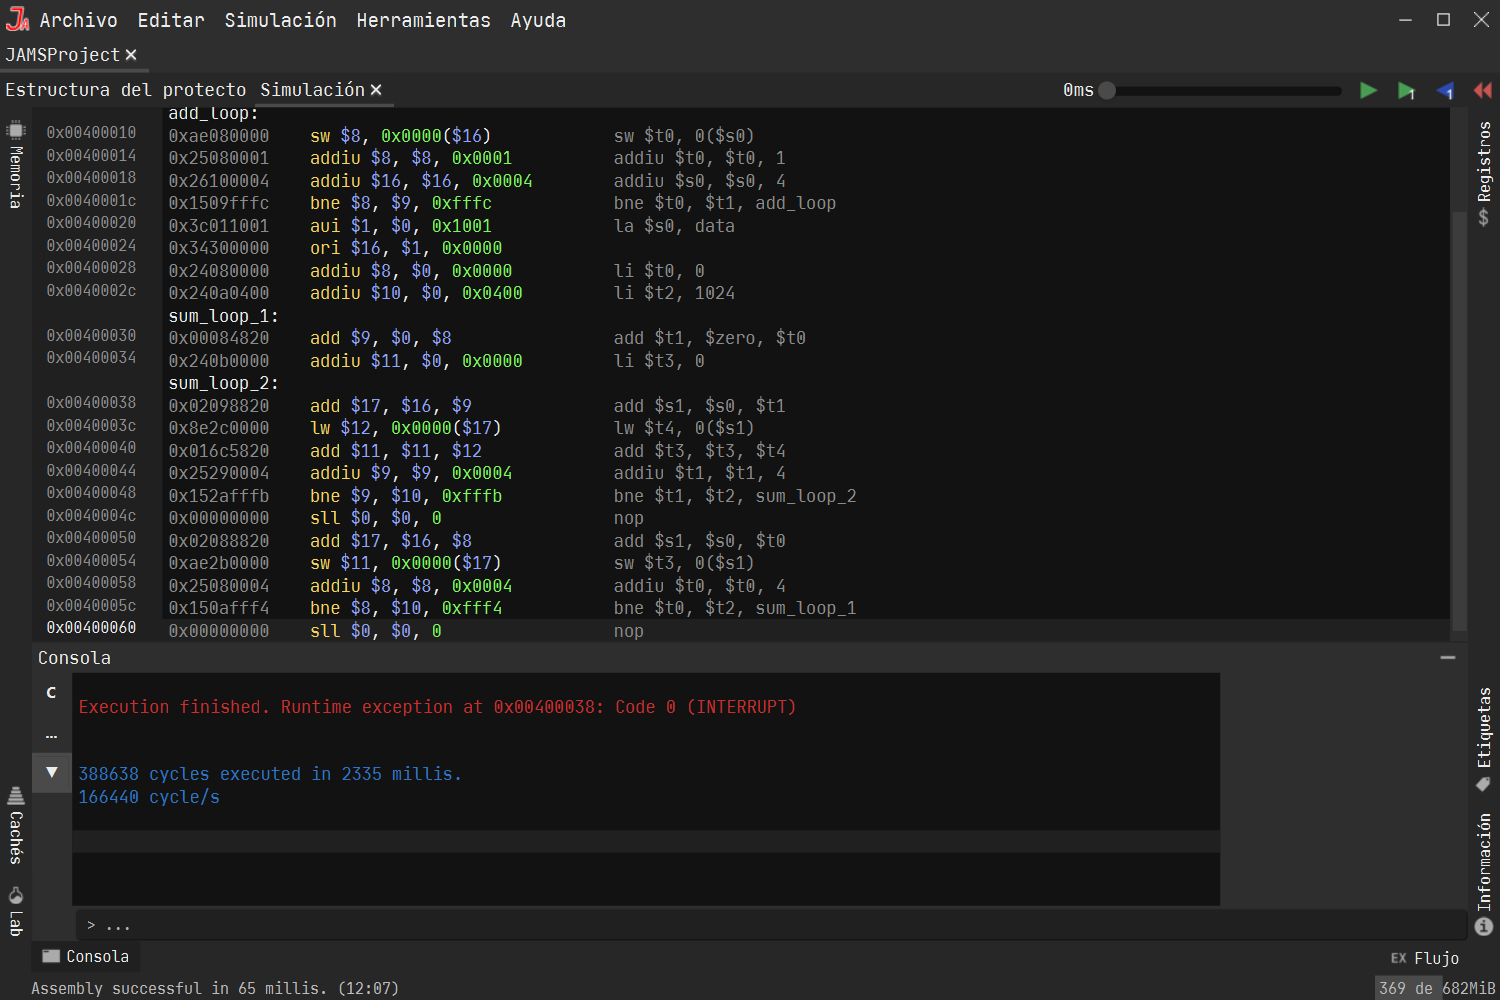
\includegraphics[width=0.8\textwidth]{images/mips/jams-exception}
    \caption{Excepción en una simulación}
    \label{fig:jams-exception}
\end{figure}

Cuando se producen varias interrupciones al mismo tiempo,
son atendidas secuencialmente, teniendo más prioridad
la interrupción \textbf{con mayor nivel}.
Si se produce una interrupción mientras el simulador está en el
modo \textit{kernel}, esta se añade a la cola de interrupciones
y se procesará cuando el simulador pase al modo usuario.

Las interrupciones pueden clasificarse en interrupciones
\textit{software} e interrupciones \textit{hardware}:
\begin{itemize}
    \item \textbf{Interrupciones \textit{software}:} permiten informar
    al programa de errores o excepciones en la simulación.
    Este tipo de interrupciones se produce por excepciones
    inherentes a la ejecución de las instrucciones que forman el programa.
    Estas interrupciones son de nivel 1.
    \item \textbf{Interrupciones \textit{hardware}:} permiten informar
    al programa de eventos generados por los diferentes componentes
    conectados al simulador.
    Estas interrupciones están definidas por
    niveles, definidos del 2 al 63.
    Estos niveles permiten calcular la dirección de memoria
    del punto de entrada del controlador de interrupciones.
\end{itemize}

El simulador gestiona las interrupciones usando la
implementación presentada en la figura \ref{fig:mips-exception-generator},
extraída del documento
\textit{MIPS® Architecture For Programmers Vol. III}\cite{MIPS_VOL_3},
permitiendo generar hasta 63 tipos diferentes de excepciones.

\begin{figure}[h]
    \centering
    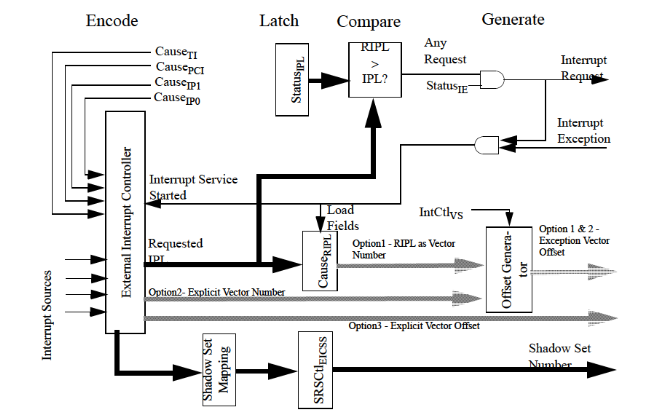
\includegraphics[width=\textwidth]{images/mips/mips-exception-generator}
    \caption{Generador de excepciones para excepciones externas}
    \label{fig:mips-exception-generator}
\end{figure}

    \chapter{Resultados}\label{ch:resultados}


\section{Resultados relativos al objetivo 1}\label{sec:resultados-relativos-al-objetivo-1}

Los resultados de este objetivo corresponden a la investigación de
tecnologías adecuadas para el desarrollo de la aplicación,
buscando un lenguaje de programación y un \textit{framework} de
desarrollo de aplicaciones de escritorio que permitan crear
aplicaciones modernas, multiplataforma, de gran calidad,
y que permitan cargar código externo a voluntad.\note{Óscar: cambiar
  aquí investigar y buscar de acuerdo a cómo quede redactado el objetivo}

Se considera que \textbf{se ha realizado una búsqueda adecuada}
del lenguaje de programación y del \textit{framework}, los cuales
terminaron siendo \textit{Java 17} y \textit{JavaFX}.
Con estas tecnologías se ha conseguido desarrollar una aplicación
moderna y multiplataforma, con soporte para componentes y totalmente
personalizable.\note{Óscar: ¡¡Uffff!! No puedes decir esto así, ni
  mucho menos: ¿métricas utilizadas para determinar que la búsqueda
  fue adecuada? ¿Quién lo asevera? ¿En qué te apoyas para decirlo?}

\begin{figure}[h]
    \centering
    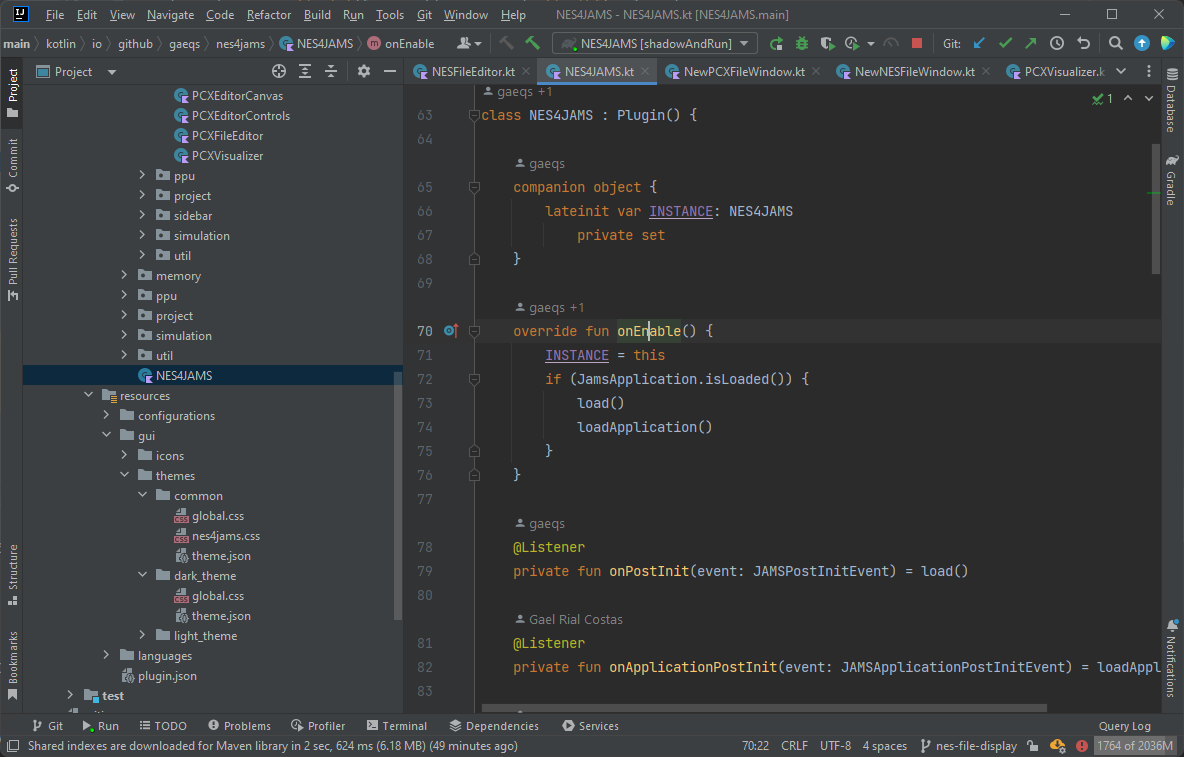
\includegraphics[width=0.8\textwidth]{images/result/idea-plugin}
    \caption{Desarrollo del componente \textit{NES4JAMS} en \textit{Kotlin}}
    \label{fig:jams-plugin}
\end{figure}

Gracias al uso de una versión de \textit{Java} moderna,
el desarrollo de la aplicación ha sido \textbf{mucho más rápido} y el resultado
ha sido \textbf{mucho más profesional}, pudiendo implementar diseños y
algoritmos rápidamente y con menores errores.
\textit{JavaFX} ha permitido desarrollar una interfaz de usuario
que se despega del conocido y desfasado formato de las aplicaciones
\textit{Swing}.
Gracias a su fácil desarrollo y su capacidad de usar código
\textit{CSS} para definir el estilo de la aplicación, \textit{JAMS}
puede presumir de tener un aspecto moderno y profesional.

Una de las ventajas que fue apareciendo durante el
desarrollo con respecto a utilizar \textit{Java} ha sido la
capacidad de poder usar otros lenguajes de programación capaces
de compilar a la \textit{JVM} para el desarrollo de componentes.
El desarrollador podrá escoger de \newODR{entre} un \textbf{amplio abanico de lenguajes}
de programación para el desarrollo de su componente.
Algunos ejemplos de lenguajes de programación que compilan a la \textit{JVM}
son \textit{Scala}, \textit{Kotlin} o \textit{Groovy}.
Un ejemplo de componente desarrollado en \textit{Kotlin} sería
\textit{NES4JAMS}, el cual es parte del Trabajo de Fin de Grado del Grado en
Diseño y Desarrollo de Videojuegos y cuyo método principal se puede observar
en la figura \ref{fig:jams-plugin}.\note{Óscar: yo esto no lo diría,
  en línea con lo que he ido comentando. Lo puedes poner como trabajos
  futuros. Al fin y al cabo, en lo que respecta a este TFG, lo es}


\section{Resultados relativos al objetivo 2}\label{sec:resultados-relativos-al-objetivo-2}

Los resultados de este objetivo corresponden a la creación de
un entorno base y un \textit{framework} que permita \textbf{implementar
diferentes entornos y herramientas}, creando así una capa
de abstracción que ayude a los desarrolladores y al propio
\textit{JAMS} a crear herramientas de manera rápida y sencilla.

Se considera que \textbf{se ha superado con creces}\note{Óscar: no
  digas con creces; se ha superado. También tenemos que hablar de esto}
el objetivo.
Gracias a las diferentes tecnologías que se han desarrollado
para la base, se pueden crear nuevas herramientas en cuestión
de minutos.
Los objetivos definidos en el Trabajo de Fin de Grado del Grado en
Diseño y Desarrollo de Videojuegos y mencionados en esta memoria
se han desarrollado paralelamente a este objetivo, resultando
en una aplicación base \textbf{robusta}, con capacidad de personalizar
una gran cantidad de aspectos del entorno.

La base también permite a los usuarios más comunes e
inexpertos personalizar el entorno de desarrollo gracias a la
\textbf{extensa configuración} y la capacidad de poder producir
\textbf{paquetes de idiomas y de temas}.
El resultado de estas personalizaciones se puede apreciar
perfectamente en la figura \ref{fig:jams-collage}.

\begin{figure}[h]
    \centering
    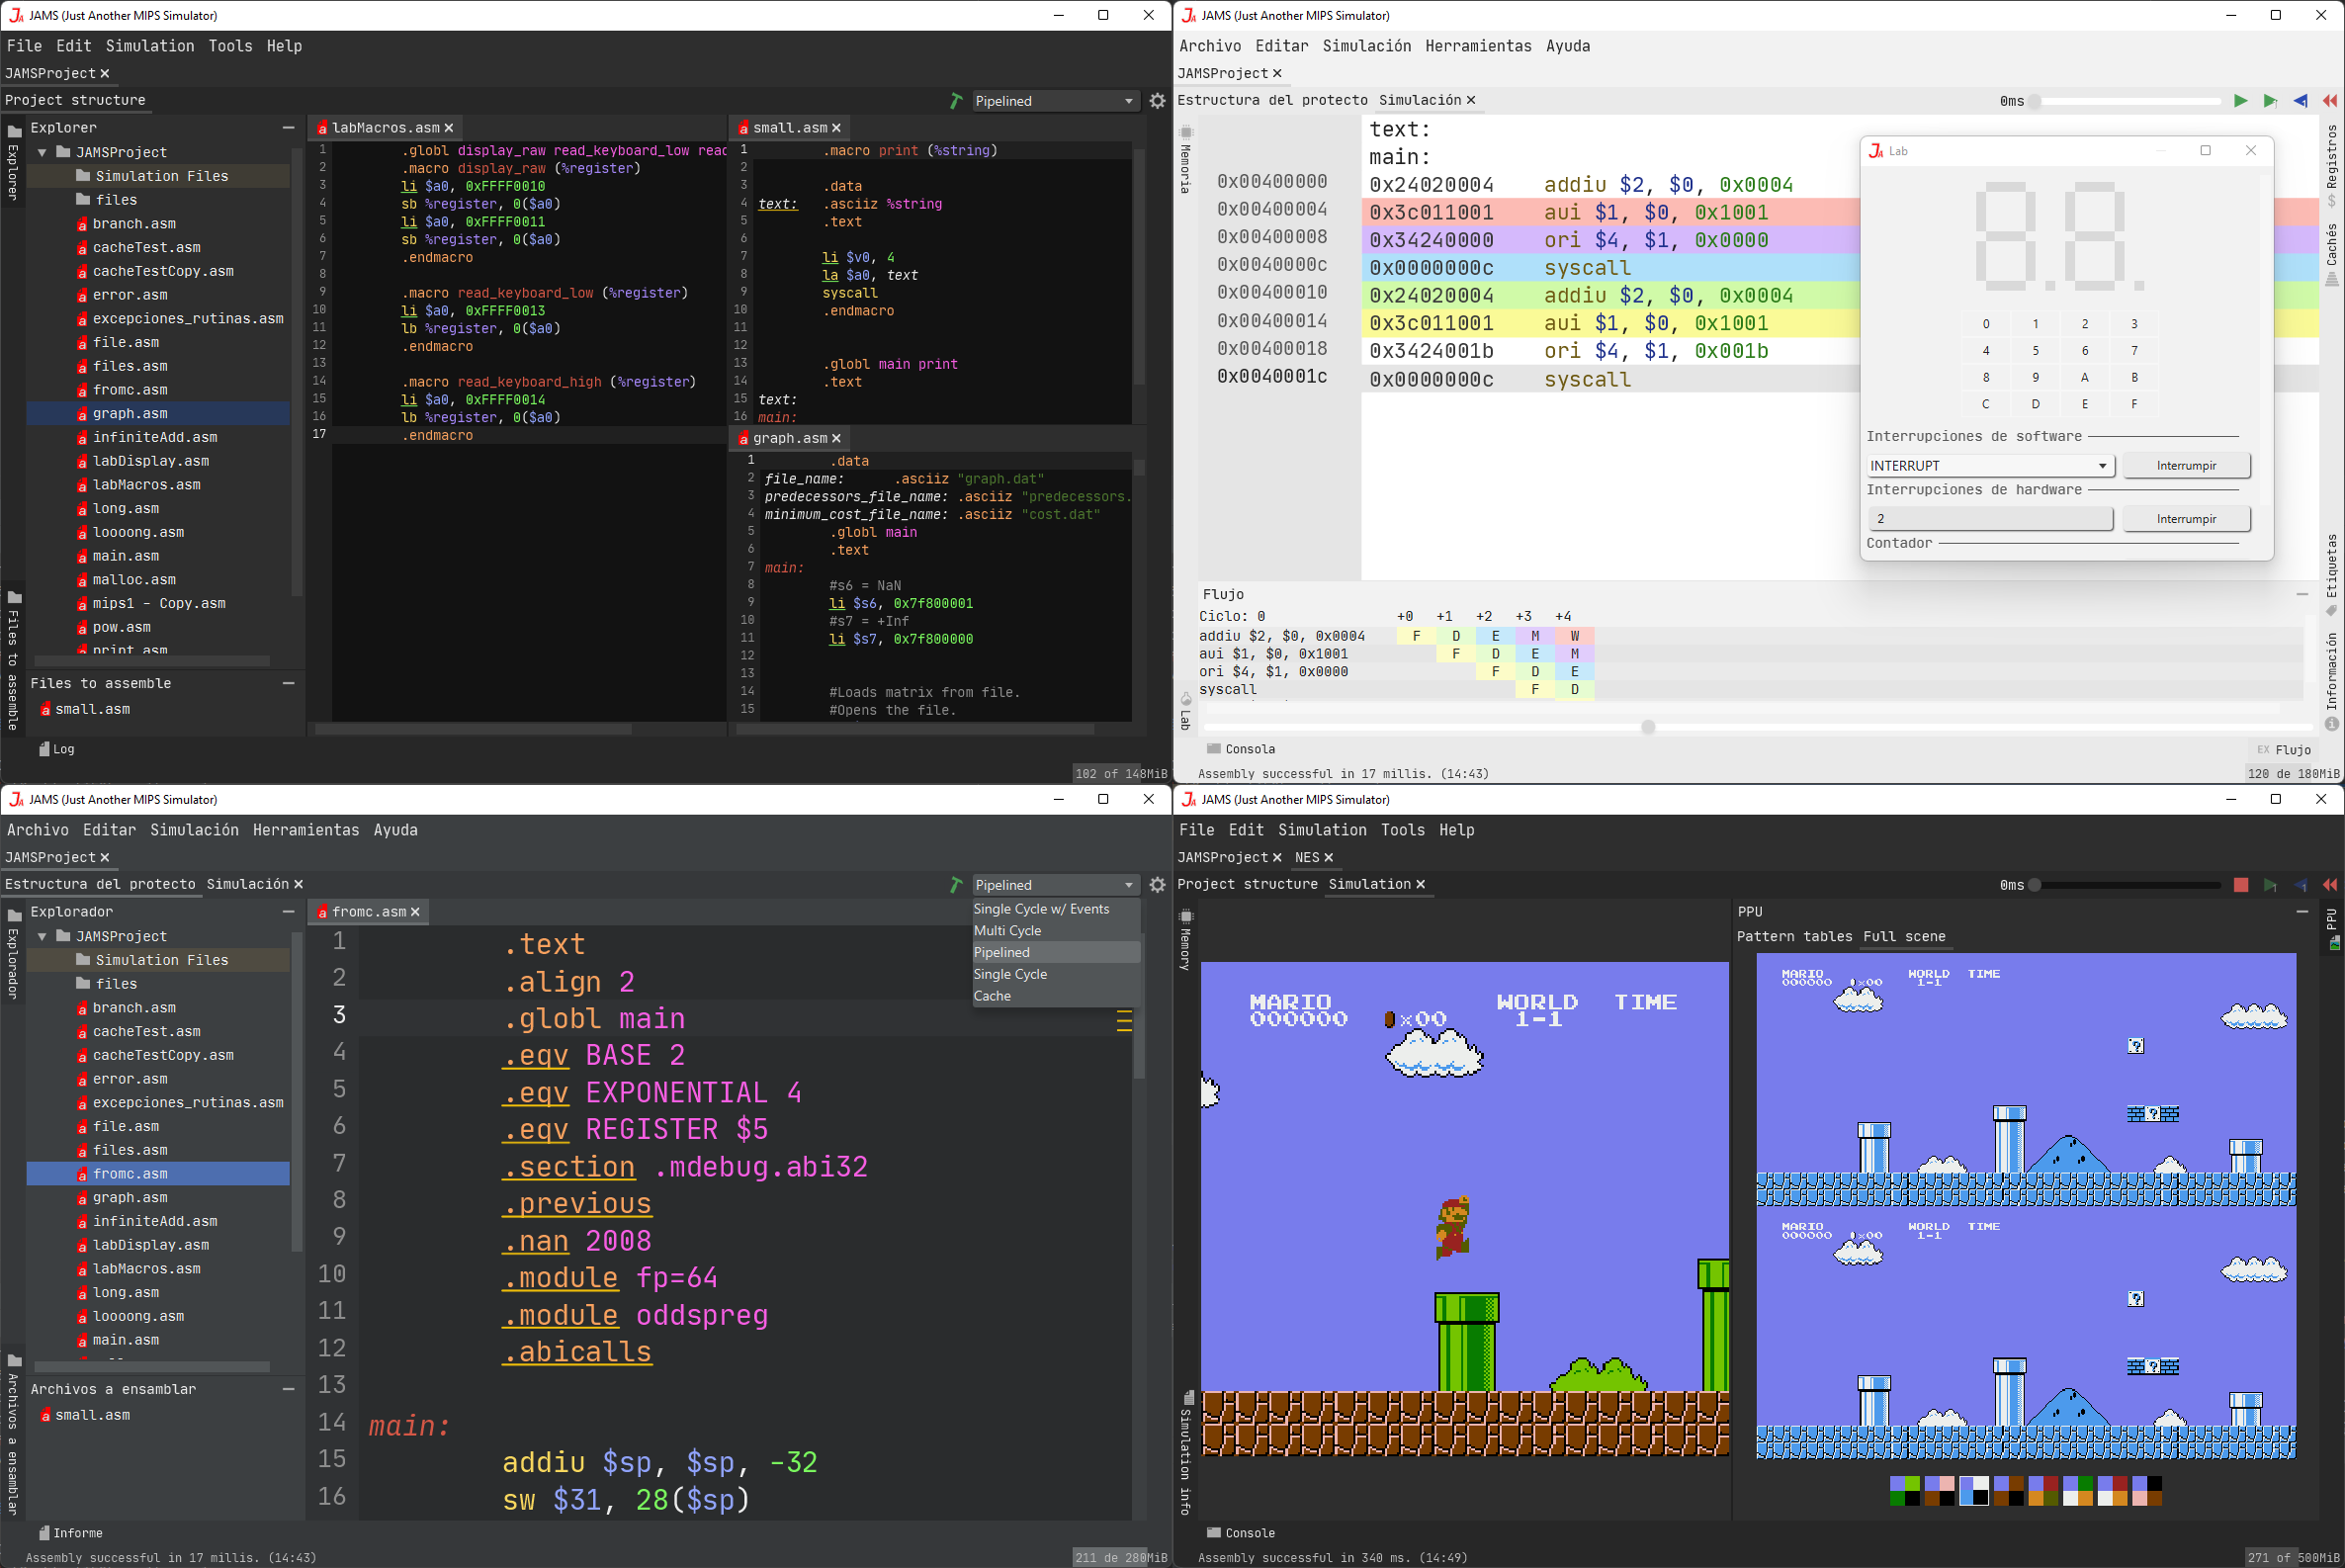
\includegraphics[width=0.8\textwidth]{images/result/jams-collage}
    \caption{Diferentes perfiles de personalización de JAMS}
    \label{fig:jams-collage}
\end{figure}

Por último, destacar el resultado de la \textit{interfaz de usuario}.
El uso de nodos como elemento central de la interfaz puede considerarse
un \textbf{acierto}: son componentes muy fáciles de usar y altamente personalizables.
Estos nodos son independientes entre sí, y muchos de ellos son \textbf{independientes}
de la tecnología que esté empleando el usuario, como es el caso del \textbf{explorador}.
Esto permite que sean herramientas \textbf{altamente reutilizables}, estando en todo
momento a disposición del desarrollador de componentes.


\section{Resultados relativos al objetivo 3}\label{sec:resultados-relativos-al-objetivo-3}

Los resultados de este objetivo corresponden al desarrollo
de un entorno de desarrollo para la arquitectura \textit{MIPS32}
usando la base creada en el objetivo anterior.
El objetivo requiere de la creación de un editor, un ensamblador
y un simulador, además de diferentes herramientas que complementen
a estos tres elementos principales.

Se considera que este objetivo se ha superado
de manera óptima.
\textit{JAMS} presenta de base un entorno de desarrollo completo
para la arquitectura \textit{MIPS32}.

El \textbf{editor de texto} está al nivel de los editores de texto
inteligentes que se pueden encontrar en los entornos de desarrollo
actuales, \textbf{ayudando al usuario} en la mayoría de las tareas
relacionadas con desarrollar una aplicación en ensamblador, como se observa
en la figura \ref{fig:mips-editor}.

\begin{figure}[h]
    \centering
    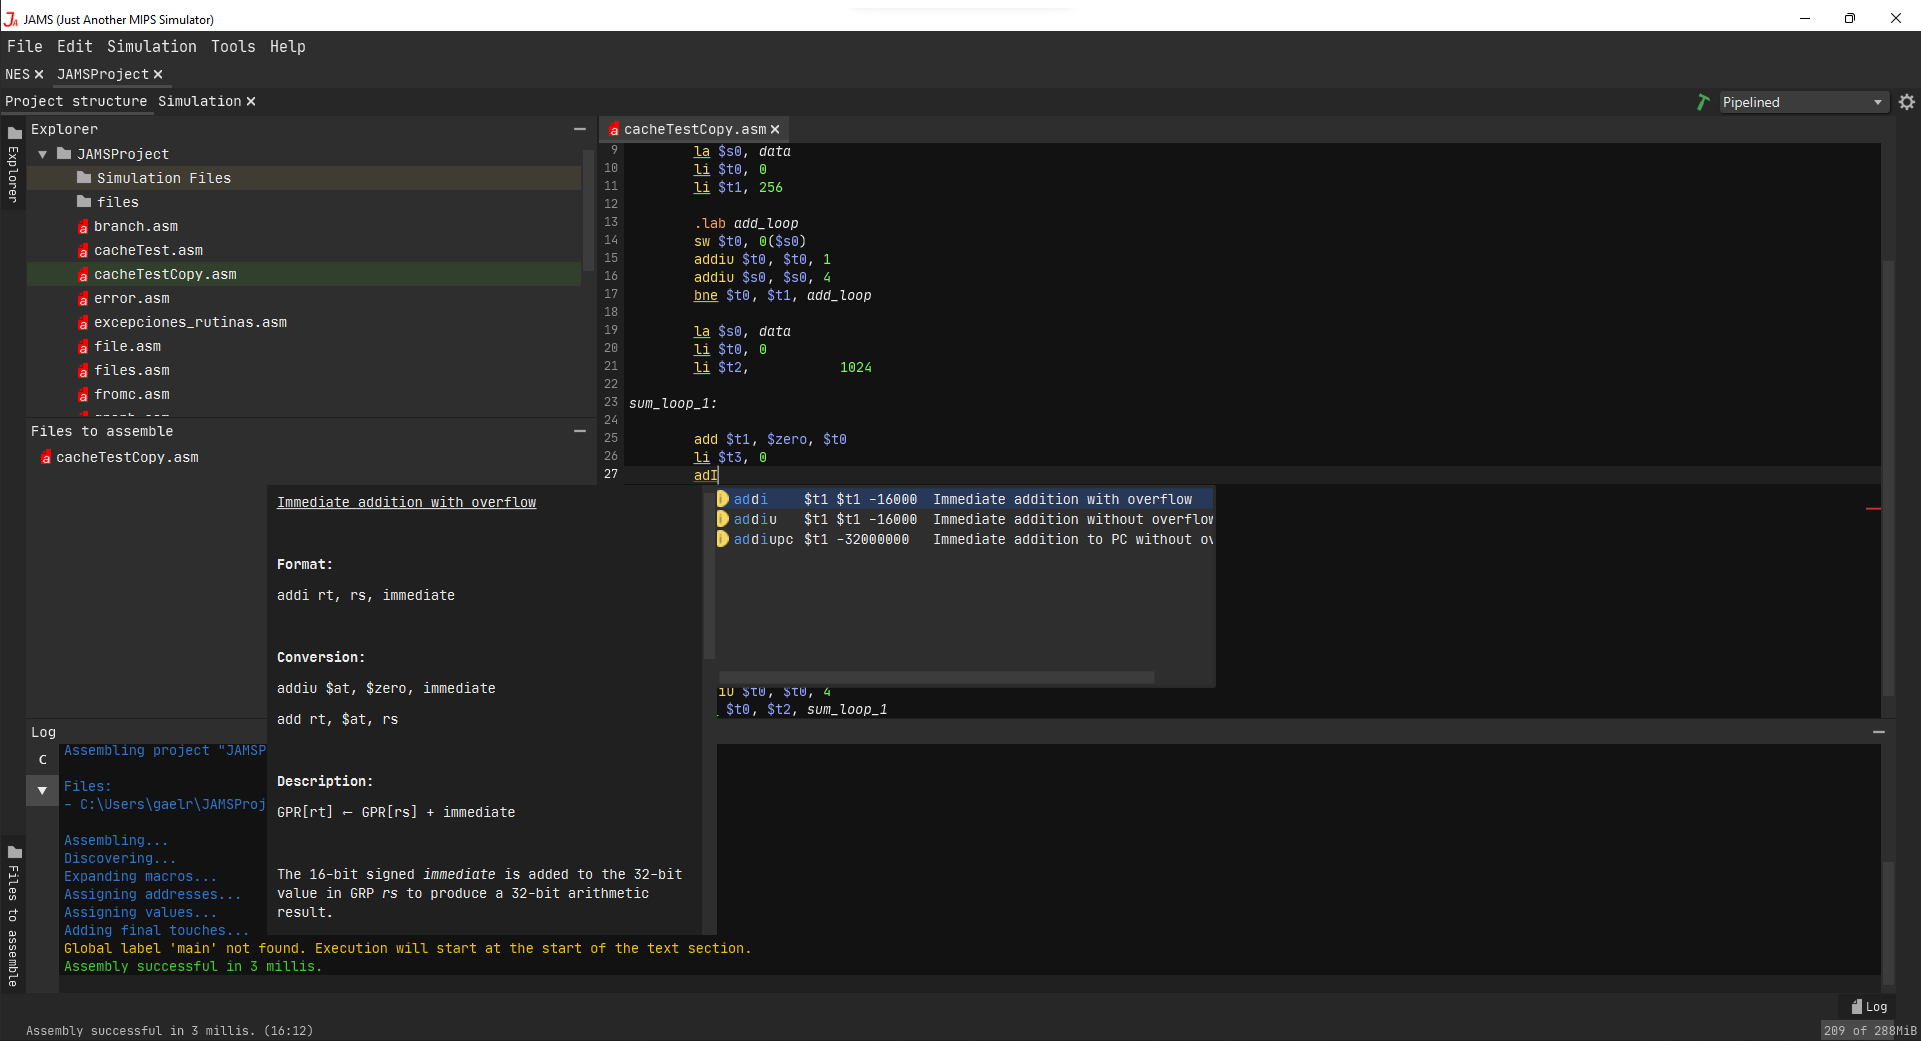
\includegraphics[width=\textwidth]{images/result/mips-editor}
    \caption{Editor de texto proporcionando ayuda al usuario}
    \label{fig:mips-editor}
\end{figure}

El \textbf{ensamblador} es altamente \textbf{personalizable},
permitiendo que otros componentes puedan aportar nuevas instrucciones y
directivas de manera sencilla.
Este ensamblador también incorpora varias \textbf{características avanzadas}
que el usuario puede usar, como son las \textbf{macros} y las
\textbf{etiquetas relativas}.

El \textbf{simulador} permite ejecutar código ensamblador
\textbf{MIPS32} en diferentes arquitecturas, siendo la arquitectura
uniciclo la más rápida de todas ellas, llegando a superar los
\textbf{40 millones de ciclos cada segundo}.
El simulador \delODR{viene}\newODR{está} altamente equipado con diversas herramientas que
permiten al usuario \textbf{visualizar y modificar} el estado del simulador
de diversas maneras, tal y como se puede observar en la figura \ref{fig:mips-tools}.
Como detalle final, el simulador presenta una estructura basada en
\textbf{hilos}, lo que evita que la aplicación se congele al ejecutar
una aplicación.

\begin{figure}[h]
    \centering
    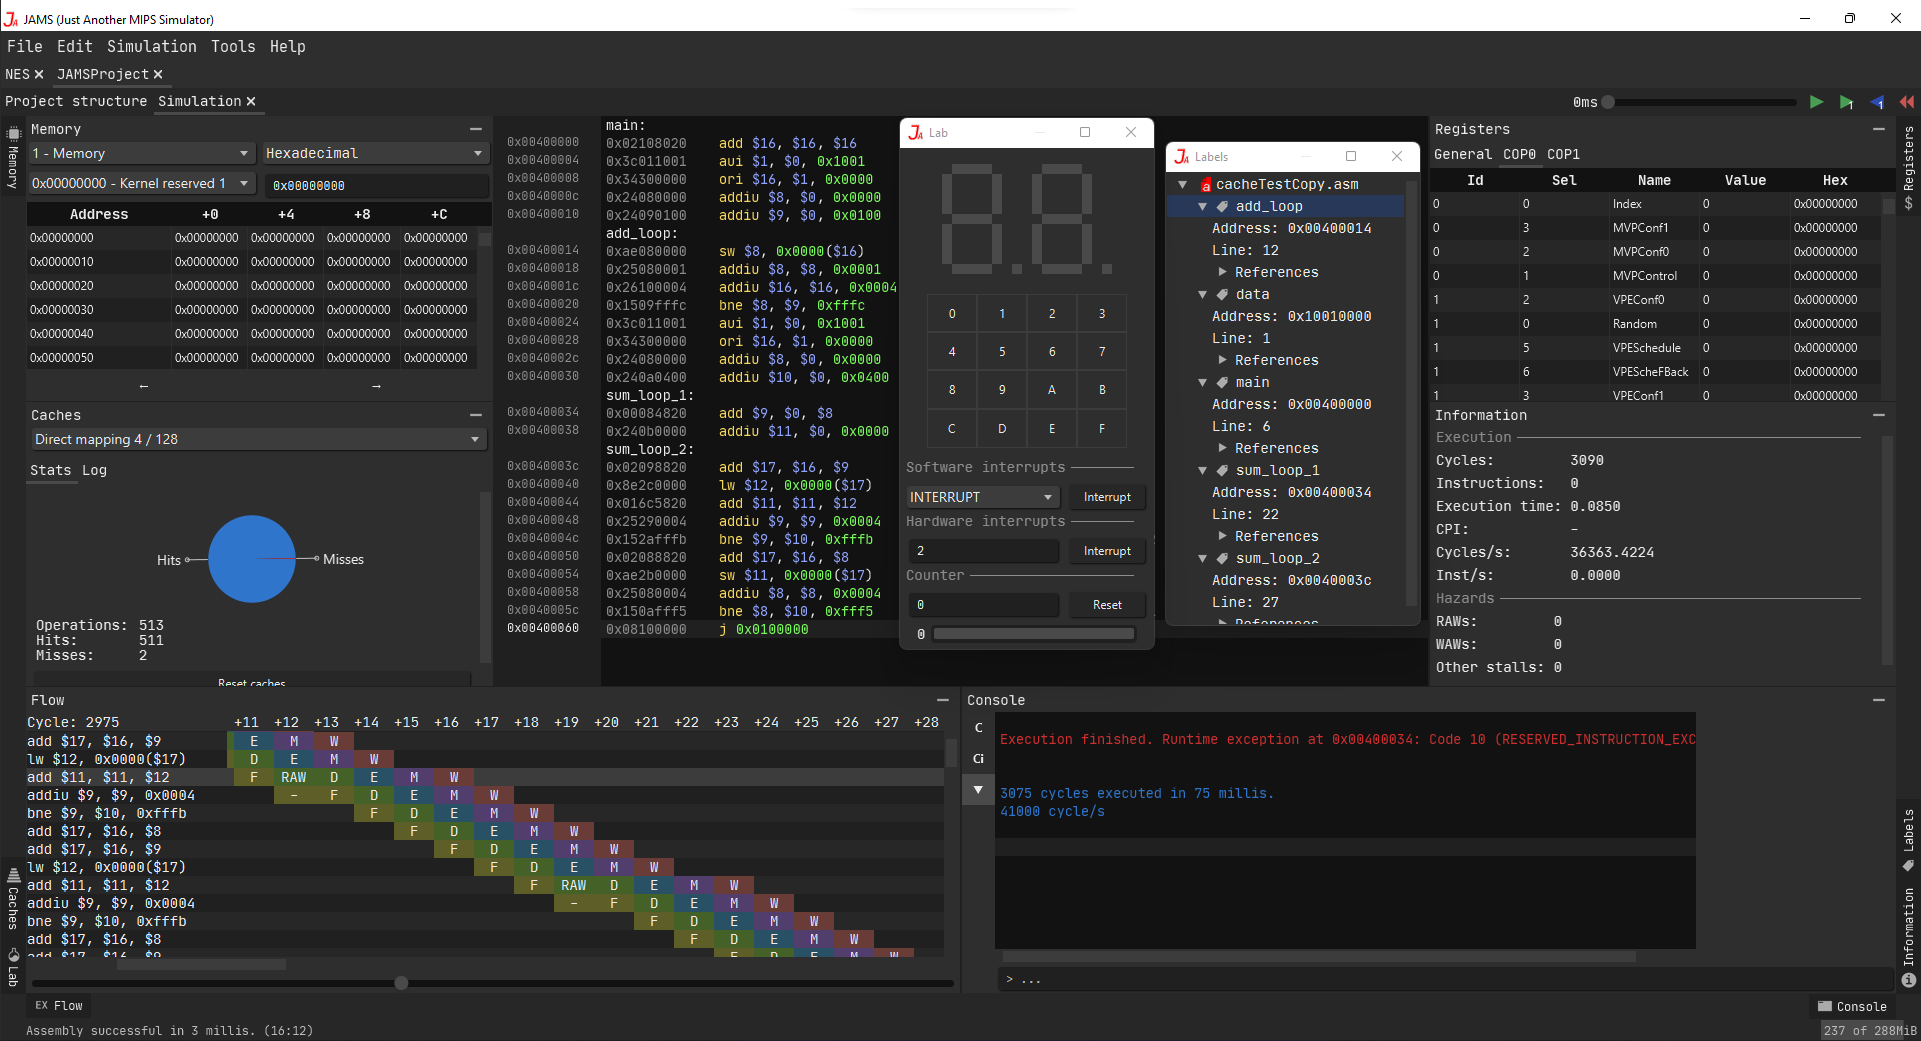
\includegraphics[width=\textwidth]{images/result/mips-tools}
    \caption{Todas las herramientas proporcionadas por el simulador}
    \label{fig:mips-tools}
\end{figure}

    \chapter{Conclusiones}\label{ch:conclusiones}

Los objetivos de este proyecto estaban asociados a la \textbf{creación
de un nuevo entorno de desarrollo} especializado en lenguajes
ensamblador que pudieran usar tanto desarrolladores avanzados
como alumnos.

\textit{JAMS} es un entorno de desarrollo moderno,
flexible, modular y fácil de usar, donde el usuario puede
crear aplicaciones de una manera rápida y cómoda,
apoyándose en las diferentes herramientas y
características que la aplicación aporta.

La aplicación viene empaquetada junto con un
editor, un ensamblador y un simulador para la arquitectura
\textit{MIPS32}, permitiendo personalizar la manera en la
que un proyecto es ejecutado.

Gracias a la buena elección de tecnologías y
\textit{frameworks}, la experiencia proporcionada por
\textit{JAMS} es altamente personalizable, permitiendo
al usuario utilizar y producir temas e idiomas.

Aunque \textit{JAMS} goce de una arquitectura
totalmente personalizable, aún no tiene la opción de cargar componentes.
Esta característica será implementada en el Trabajo de Fin de
Grado del Grado en Diseño y Desarrollo de Videojuegos.

\section{Limitaciones}\label{sec:limitaciones}

\textit{JAMS} presenta las siguientes limitaciones:

\begin{itemize}
    \item \textbf{Velocidad}: \textit{JAMS} es capaz de ejecutar
    una simulación a un máximo de \textbf{40 millones de instrucciones por segundo} en un
    procesador \textit{AMD Ryzen 7 2700X}.
    Esta velocidad, aunque supere con creces a la mayoría de simuladores \textit{MIPS32},
    puede impedir ejecutar aplicaciones que requieran de una gran capacidad de cómputo.
    \item \textbf{Soporte para MIPS32r5}: actualmente, \textit{JAMS} solo da soporte
    a la última revisión de la arquitectura \textit{MIPS32}.
    Muchos usuarios siguen utilizando la revisión anterior, por lo que tendrán que migrar
    sus proyectos antes de poder emplear \textit{JAMS}.
\end{itemize}

\section{Líneas futuras}\label{sec:líneas-futuras}

\textit{JAMS} contará con dos actualizaciones importantes en el
futuro cercano.
La primera actualización ya está en desarrollo, mientras que la
segunda actualización requerirá de nueva tecnología que
el equipo de \textit{JAVA} está desarrollando.
\begin{itemize}
    \item \textbf{Soporte para la arquitectura \textit{MIPS32r5}}:
    actualmente, \textit{JAMS} solo soporta proyectos de la revisión 6
    de la arquitectura \textit{MIPS32}.
    Esta revisión cambia la arquitectura en muchos aspectos con respecto
    a la revisión anterior, lo que fuerza a muchas personas a tener
    que migrar gran parte del código de sus proyectos.
    Añadir soporte a la revisión 5 será una tarea relativamente sencilla,
    sabiendo que la revisión 6 añade más características de las que quita.
    \item \textbf{Uso del \textit{Proyecto Valhalla}:} el
    \textit{Proyecto Valhalla}\cite{PROJECT_VALHALLA}, creado en 2014,
    está desarrollando una de las características más esperadas
    por los desarrolladores \textit{JAVA}: \textbf{paso por valor}.
    Esta característica permitirá optimizar de manera considerable
    muchos aspectos de \textit{JAMS}, como son el editor o el simulador.
    Estas nuevas características empezarán su desarrollo cuando esta
    tecnología esté en fase \textit{preview}.
\end{itemize}

\section{Reflexiones finales}\label{sec:reflexiones-finales}

Este ha sido el proyecto más complejo en el que he trabajo:
\textit{JAMS} abarca un montón de conceptos y tecnologías,
desde la simulación de arquitecturas hasta el despliegue de
aplicaciones automatizado, pasando por el renderizado a tiempo
real, la creación de interfaces y la estructuración de un
proyecto grande.

\textit{JAMS} ha sido una apuesta, un proyecto
que podría haberse derrumbado rápidamente.
Puede considerarse la consolidación de todos los conocimientos
que he adquirido en los últimos años, tanto fuera como dentro
de la universidad.

Finalmente, agradecer a todas las personas que me han
estado apoyando en este proyecto, a mi familia, amigos y a mis
tutores Óscar y Luis, ya que gracias a ellos este trabajo
ha sido posible.
    \printbibliography[title=Bibliografía]
\end{document}
